% !TeX encoding = UTF-8
% !TeX program = xelatex
% !TeX spellcheck = en_US

\documentclass[degree=master, degree-type=professional, fontset=mac]{thuthesis}
  % 学位 degree:
  %   doctor | master | bachelor | postdoc
  % 学位类型 degree-type:
  %   academic(默认)| professional
  % 语言 language
  %   chinese(默认)| english
  % 字体库 fontset
  %   windows | mac | fandol | ubuntu
  % 建议终版使用 Windows 平台的字体编译


% 论文基本配置,加载宏包等全局配置
% !TeX root = ./thuthesis-example.tex

% 论文基本信息配置

\thusetup{
  %******************************
  % 注意:
  %   1. 配置里面不要出现空行
  %   2. 不需要的配置信息可以删除
  %   3. 建议先阅读文档中所有关于选项的说明
  %******************************
  %
  % 输出格式
  %   选择打印版(print)或用于提交的电子版(electronic),前者会插入空白页以便直接双面打印
  %
  output = print,
  %
  % 标题
  %   可使用“\\”命令手动控制换行
  %
  title  = {面向基于图近似近邻搜索架构的\\高效算法设计},
  title* = {Efficient Algorithm Design for Graph-based Approximate Neighbor Search Architecture},
  %
  % 学位
  %   1. 学术型
  %      - 中文
  %        需注明所属的学科门类,例如:
  %        哲学、经济学、法学、教育学、文学、历史学、理学、工学、农学、医学、
  %        军事学、管理学、艺术学
  %      - 英文
  %        博士:Doctor of Philosophy
  %        硕士:
  %          哲学、文学、历史学、法学、教育学、艺术学门类,公共管理学科
  %          填写“Master of Arts“,其它填写“Master of Science”
  %   2. 专业型
  %      直接填写专业学位的名称,例如:
  %      教育博士、工程硕士等
  %      Doctor of Education, Master of Engineering
  %   3. 本科生不需要填写
  %
  degree-name  = {工程硕士},
  degree-name* = {Master of Engineering},
  %
  % 培养单位
  %   填写所属院系的全名
  %
  department = {电子工程系},
  %
  % 学科
  %   1. 学术型学位
  %      获得一级学科授权的学科填写一级学科名称,其他填写二级学科名称
  %   2. 工程硕士
  %      工程领域名称
  %   3. 其他专业型学位
  %      不填写此项
  %   4. 本科生填写专业名称,第二学位论文需标注“(第二学位)”
  %
  discipline  = {电子信息},
  discipline* = {Electronic Information},
  %
  % 姓名
  %
  author  = {刘军},
  author* = {Liu Jun},
  %
  % 指导教师
  %   中文姓名和职称之间以英文逗号“,”分开,下同
  %
  supervisor  = {汪玉, 教授},
  supervisor* = {Professor Wang Yu},
  %
  % 副指导教师
  %
  % associate-supervisor  = {陈文光, 教授},
  % associate-supervisor* = {Professor Chen Wenguang},
  %
  % 联合指导教师
  %
  % co-supervisor  = {某某某, 教授},
  % co-supervisor* = {Professor Mou Moumou},
  %
  % 日期
  %   使用 ISO 格式;默认为当前时间
  %
  % date = {2019-07-07},
  %
  % 是否在中文封面后的空白页生成书脊(默认 false)
  %
  include-spine = false,
  %
  % 密级和年限
  %   秘密, 机密, 绝密
  %
  % secret-level = {秘密},
  % secret-year  = {10},
  %
  % 博士后专有部分
  %
  % clc                = {分类号},
  % udc                = {UDC},
  % id                 = {编号},
  % discipline-level-1 = {计算机科学与技术},  % 流动站(一级学科)名称
  % discipline-level-2 = {系统结构},          % 专业(二级学科)名称
  % start-date         = {2011-07-01},        % 研究工作起始时间
}

% 载入所需的宏包

% 定理类环境宏包
\usepackage{amsthm}
% 也可以使用 ntheorem
% \usepackage[amsmath,thmmarks,hyperref]{ntheorem}

\thusetup{
  %
  % 数学字体
  % math-style = GB,  % GB | ISO | TeX
  math-font  = xits,  % stix | xits | libertinus
}

% 可以使用 nomencl 生成符号和缩略语说明
% \usepackage{nomencl}
% \makenomenclature

% 表格加脚注
\usepackage{threeparttable}

% 表格中支持跨行
\usepackage{multirow}

% 固定宽度的表格。
% \usepackage{tabularx}

% 跨页表格
\usepackage{longtable}

% 算法
\usepackage{algorithm}
\usepackage{algorithmic}

% 量和单位
\usepackage{siunitx}

% 参考文献使用 BibTeX + natbib 宏包
% 顺序编码制
\usepackage[sort]{natbib}
\bibliographystyle{thuthesis-numeric}

% 著者-出版年制
% \usepackage{natbib}
% \bibliographystyle{thuthesis-author-year}

% 本科生参考文献的著录格式
% \usepackage[sort]{natbib}
% \bibliographystyle{thuthesis-bachelor}

% 参考文献使用 BibLaTeX 宏包
% \usepackage[style=thuthesis-numeric]{biblatex}
% \usepackage[style=thuthesis-author-year]{biblatex}
% \usepackage[style=apa]{biblatex}
% \usepackage[style=mla-new]{biblatex}
% 声明 BibLaTeX 的数据库
% \addbibresource{ref/refs.bib}

% 定义所有的图片文件在 figures 子目录下
\graphicspath{{figures/}}

% 自定义命令
\newcommand\todo[1]{\textcolor{red}{TODO: #1}}
\newcommand\ganns{基于图的近似近邻搜索}

% 数学命令
\makeatletter
\newcommand\dif{%  % 微分符号
  \mathop{}\!%
  \ifthu@math@style@TeX
    d%
  \else
    \mathrm{d}%
  \fi
}
\makeatother

% hyperref 宏包在最后调用
\usepackage{hyperref}



\begin{document}

% 封面
\maketitle

% 学位论文指导小组、公开评阅人和答辩委员会名单
% 本科生不需要
% !TeX root = ../main.tex

\begin{committee}[name={学位论文指导小组、公开评阅人和答辩委员会名单}]

  \newcolumntype{C}[1]{@{}>{\centering\arraybackslash}p{#1}}

  \section*{指导小组名单}

  \begin{center}
    \begin{tabular}{C{3cm}C{3cm}C{9cm}@{}}
      李XX & 教授     & 清华大学 \\
      王XX & 副教授   & 清华大学 \\
      张XX & 助理教授 & 清华大学 \\
    \end{tabular}
  \end{center}


  \section*{公开评阅人名单}

  \begin{center}
    \begin{tabular}{C{3cm}C{3cm}C{9cm}@{}}
      刘XX & 教授   & 清华大学                    \\
      陈XX & 副教授 & XXXX大学                    \\
      杨XX & 研究员 & 中国XXXX科学院XXXXXXX研究所 \\
    \end{tabular}
  \end{center}


  \section*{答辩委员会名单}

  \begin{center}
    \begin{tabular}{C{2.75cm}C{2.98cm}C{4.63cm}C{4.63cm}@{}}
      主席 & 赵XX                  & 教授                    & 清华大学       \\
      委员 & 刘XX                  & 教授                    & 清华大学       \\
          & \multirow{2}{*}{杨XX} & \multirow{2}{*}{研究员} & 中国XXXX科学院 \\
          &                       &                         & XXXXXXX研究所  \\
          & 黄XX                  & 教授                    & XXXX大学       \\
          & 周XX                  & 副教授                  & XXXX大学       \\
      秘书 & 吴XX                  & 助理研究员              & 清华大学       \\
    \end{tabular}
  \end{center}

\end{committee}



% 也可以导入 Word 版转的 PDF 文件
% \begin{committee}[file=figures/committee.pdf]
% \end{committee}


% 使用授权的说明
\copyrightpage
% 将签字扫描后授权文件 scan-copyright.pdf 替换原始页面
% \copyrightpage[file=scan-copyright.pdf]

\frontmatter
% !TeX root = ../main.tex

% 中英文摘要和关键字

\begin{abstract}
  推荐系统目前被广泛使用到各类场景,例如电商、社交、广告等等。其中推荐系统的核心组件之一是近似近邻搜索算法,该算法的目的是从百万上亿的数据中检索与给定查询最相似的结果。其中基于图结构的近似近邻搜索算法在多个公开基准上的测试都优于其他类型的算法,而被广泛适用于推荐系统中,作为推荐系统的核心组件之一。本文以推荐系统作为近似近邻搜索的典型场景,开展面向\textbf{图结构推荐算法}和硬件架构的软硬件协同设计研究。随着大数据时代的快速到来,推荐系统所需要处理的数据量也急剧增长,图结构推荐算法在算法和硬件层面也都面临新的问题和挑战。因此,本文以推荐系统作为近似近邻搜索算法的典型场景,从算法、架构和系统三个层面开展面向图结构推荐算法和硬件架构的软硬件协同设计研究。

  在算法层面,在各类近似近邻搜索算法中,尽管图结构推荐算法拥有出色的搜索性能,但是面临构建开销大和搜索时存在冗余的问题。本文针对这两个问题分别提出了构建时优化和搜算阶段的分析,指出冗余的原因是由于图结构中不同区域的连接关系不同所导致。

  在架构层面,图结构推荐算法在现有硬件架构上(如CPU和GPU)面临执行能效低下的问题。其核心原因是图结构引入大量的间接索引问题,导致现有的冯诺依曼这种存算分离的架构在数据传输的开销很大。因此本文提出了一种DRAM-SSD的层次化近存储处理架构,是一个针对图结构推荐算法所设计的高效硬件处理架构。

  在系统层面,随着数据规模的增加,拓展性是一个必须要考虑的问题。由于节点间通信的昂贵开销,现有多机方案都采用节点间无通信的方案,但是这种方案受到图结构的影响导致很差的拓展性。因此,本文在系统层次进一步提出了可拓展的处理方案,并在FPGA上进行了功能验证,取得了超过近存储架构设计的性能。

  % 关键词用“英文逗号”分隔,输出时会自动处理为正确的分隔符
  \thusetup{
    keywords = {推荐系统, 近似近邻搜索, 软硬件协同设计, 近存储计算},
  }
\end{abstract}

\begin{abstract*}
  TODO

  % Use comma as separator when inputting
  \thusetup{
    keywords* = {Recommendation system, approximate nearest neighbor search, software-hardware co-design, near-memory computing},
  }
\end{abstract*}


% 目录
\tableofcontents

% 插图和附表清单
% 本科生的插图索引和表格索引需要移至正文之后、参考文献前
% \listoffiguresandtables  % 插图和附表清单(仅限研究生)
\listoffigures           % 插图清单
\listoftables            % 附表清单

% 符号对照表
% !TeX root = ../main.tex

\begin{denotation}[3cm]
  \item[PI] 聚酰亚胺
  \item[MPI] 聚酰亚胺模型化合物,N-苯基邻苯酰亚胺
  \item[PBI] 聚苯并咪唑
  \item[MPBI] 聚苯并咪唑模型化合物,N-苯基苯并咪唑
  \item[PY] 聚吡咙
  \item[PMDA-BDA] 均苯四酸二酐与联苯四胺合成的聚吡咙薄膜
  \item[MPY] 聚吡咙模型化合物
  \item[As-PPT] 聚苯基不对称三嗪
  \item[MAsPPT] 聚苯基不对称三嗪单模型化合物,3,5,6-三苯基-1,2,4-三嗪
  \item[DMAsPPT] 聚苯基不对称三嗪双模型化合物(水解实验模型化合物)
  \item[S-PPT] 聚苯基对称三嗪
  \item[MSPPT] 聚苯基对称三嗪模型化合物,2,4,6-三苯基-1,3,5-三嗪
  \item[PPQ] 聚苯基喹噁啉
  \item[MPPQ] 聚苯基喹噁啉模型化合物,3,4-二苯基苯并二嗪
  \item[HMPI] 聚酰亚胺模型化合物的质子化产物
  \item[HMPY] 聚吡咙模型化合物的质子化产物
  \item[HMPBI] 聚苯并咪唑模型化合物的质子化产物
  \item[HMAsPPT] 聚苯基不对称三嗪模型化合物的质子化产物
  \item[HMSPPT] 聚苯基对称三嗪模型化合物的质子化产物
  \item[HMPPQ] 聚苯基喹噁啉模型化合物的质子化产物
  \item[PDT] 热分解温度
  \item[HPLC] 高效液相色谱(High Performance Liquid Chromatography)
  \item[HPCE] 高效毛细管电泳色谱(High Performance Capillary lectrophoresis)
  \item[LC-MS] 液相色谱-质谱联用(Liquid chromatography-Mass Spectrum)
  \item[TIC] 总离子浓度(Total Ion Content)
  \item[\textit{ab initio}] 基于第一原理的量子化学计算方法,常称从头算法
  \item[DFT] 密度泛函理论(Density Functional Theory)
  \item[$E_a$] 化学反应的活化能(Activation Energy)
  \item[ZPE] 零点振动能(Zero Vibration Energy)
  \item[PES] 势能面(Potential Energy Surface)
  \item[TS] 过渡态(Transition State)
  \item[TST] 过渡态理论(Transition State Theory)
  \item[$\increment G^\neq$] 活化自由能(Activation Free Energy)
  \item[$\kappa$] 传输系数(Transmission Coefficient)
  \item[IRC] 内禀反应坐标(Intrinsic Reaction Coordinates)
  \item[$\nu_i$] 虚频(Imaginary Frequency)
  \item[ONIOM] 分层算法(Our own N-layered Integrated molecular Orbital and molecular Mechanics)
  \item[SCF] 自洽场(Self-Consistent Field)
  \item[SCRF] 自洽反应场(Self-Consistent Reaction Field)
\end{denotation}



% 也可以使用 nomencl 宏包,需要在导言区
% \usepackage{nomencl}
% \makenomenclature

% 在这里输出符号说明
% \printnomenclature[3cm]

% 在正文中的任意为都可以标题
% \nomenclature{PI}{聚酰亚胺}
% \nomenclature{MPI}{聚酰亚胺模型化合物,N-苯基邻苯酰亚胺}
% \nomenclature{PBI}{聚苯并咪唑}
% \nomenclature{MPBI}{聚苯并咪唑模型化合物,N-苯基苯并咪唑}
% \nomenclature{PY}{聚吡咙}
% \nomenclature{PMDA-BDA}{均苯四酸二酐与联苯四胺合成的聚吡咙薄膜}
% \nomenclature{MPY}{聚吡咙模型化合物}
% \nomenclature{As-PPT}{聚苯基不对称三嗪}
% \nomenclature{MAsPPT}{聚苯基不对称三嗪单模型化合物,3,5,6-三苯基-1,2,4-三嗪}
% \nomenclature{DMAsPPT}{聚苯基不对称三嗪双模型化合物(水解实验模型化合物)}
% \nomenclature{S-PPT}{聚苯基对称三嗪}
% \nomenclature{MSPPT}{聚苯基对称三嗪模型化合物,2,4,6-三苯基-1,3,5-三嗪}
% \nomenclature{PPQ}{聚苯基喹噁啉}
% \nomenclature{MPPQ}{聚苯基喹噁啉模型化合物,3,4-二苯基苯并二嗪}
% \nomenclature{HMPI}{聚酰亚胺模型化合物的质子化产物}
% \nomenclature{HMPY}{聚吡咙模型化合物的质子化产物}
% \nomenclature{HMPBI}{聚苯并咪唑模型化合物的质子化产物}
% \nomenclature{HMAsPPT}{聚苯基不对称三嗪模型化合物的质子化产物}
% \nomenclature{HMSPPT}{聚苯基对称三嗪模型化合物的质子化产物}
% \nomenclature{HMPPQ}{聚苯基喹噁啉模型化合物的质子化产物}
% \nomenclature{PDT}{热分解温度}
% \nomenclature{HPLC}{高效液相色谱(High Performance Liquid Chromatography)}
% \nomenclature{HPCE}{高效毛细管电泳色谱(High Performance Capillary lectrophoresis)}
% \nomenclature{LC-MS}{液相色谱-质谱联用(Liquid chromatography-Mass Spectrum)}
% \nomenclature{TIC}{总离子浓度(Total Ion Content)}
% \nomenclature{\textit{ab initio}}{基于第一原理的量子化学计算方法,常称从头算法}
% \nomenclature{DFT}{密度泛函理论(Density Functional Theory)}
% \nomenclature{$E_a$}{化学反应的活化能(Activation Energy)}
% \nomenclature{ZPE}{零点振动能(Zero Vibration Energy)}
% \nomenclature{PES}{势能面(Potential Energy Surface)}
% \nomenclature{TS}{过渡态(Transition State)}
% \nomenclature{TST}{过渡态理论(Transition State Theory)}
% \nomenclature{$\increment G^\neq$}{活化自由能(Activation Free Energy)}
% \nomenclature{$\kappa$}{传输系数(Transmission Coefficient)}
% \nomenclature{IRC}{内禀反应坐标(Intrinsic Reaction Coordinates)}
% \nomenclature{$\nu_i$}{虚频(Imaginary Frequency)}
% \nomenclature{ONIOM}{分层算法(Our own N-layered Integrated molecular Orbital and molecular Mechanics)}
% \nomenclature{SCF}{自洽场(Self-Consistent Field)}
% \nomenclature{SCRF}{自洽反应场(Self-Consistent Reaction Field)}



% 正文部分
\mainmatter
% !TeX root = ../main.tex

\chapter{引言}

\section{研究背景与意义}
% 推荐系统很重要
推荐系统是基于用户的兴趣爱好,从海量候选集中帮助用户找到感兴趣的内容\cite{li2020collaborative, dhelim2020personality}。推荐系统的应用场景非常广泛,包括社交推荐\cite{li2014social, tang2013social}、商品推荐(电商)\cite{zhang2012research, wu2008clustering}、长短视频推荐\cite{davidson2010youtube, hongliang2015video}和新闻推荐\cite{li2011scene, zihayat2019utility}等等。从商业价值角度来看,推荐系统具有极高的商业价值,如图~\ref{fig:apps}所示,大量应用使用到推荐系统。例如阿里巴巴旗下的电商平台淘宝\cite{gong2020edgerec}、快手短视频\cite{cai2023reinforcing}、字节跳动旗下的抖音短视频、腾讯旗下以社交平台微信为核心的众多业务平台等等。

\begin{figure}
  \centering
  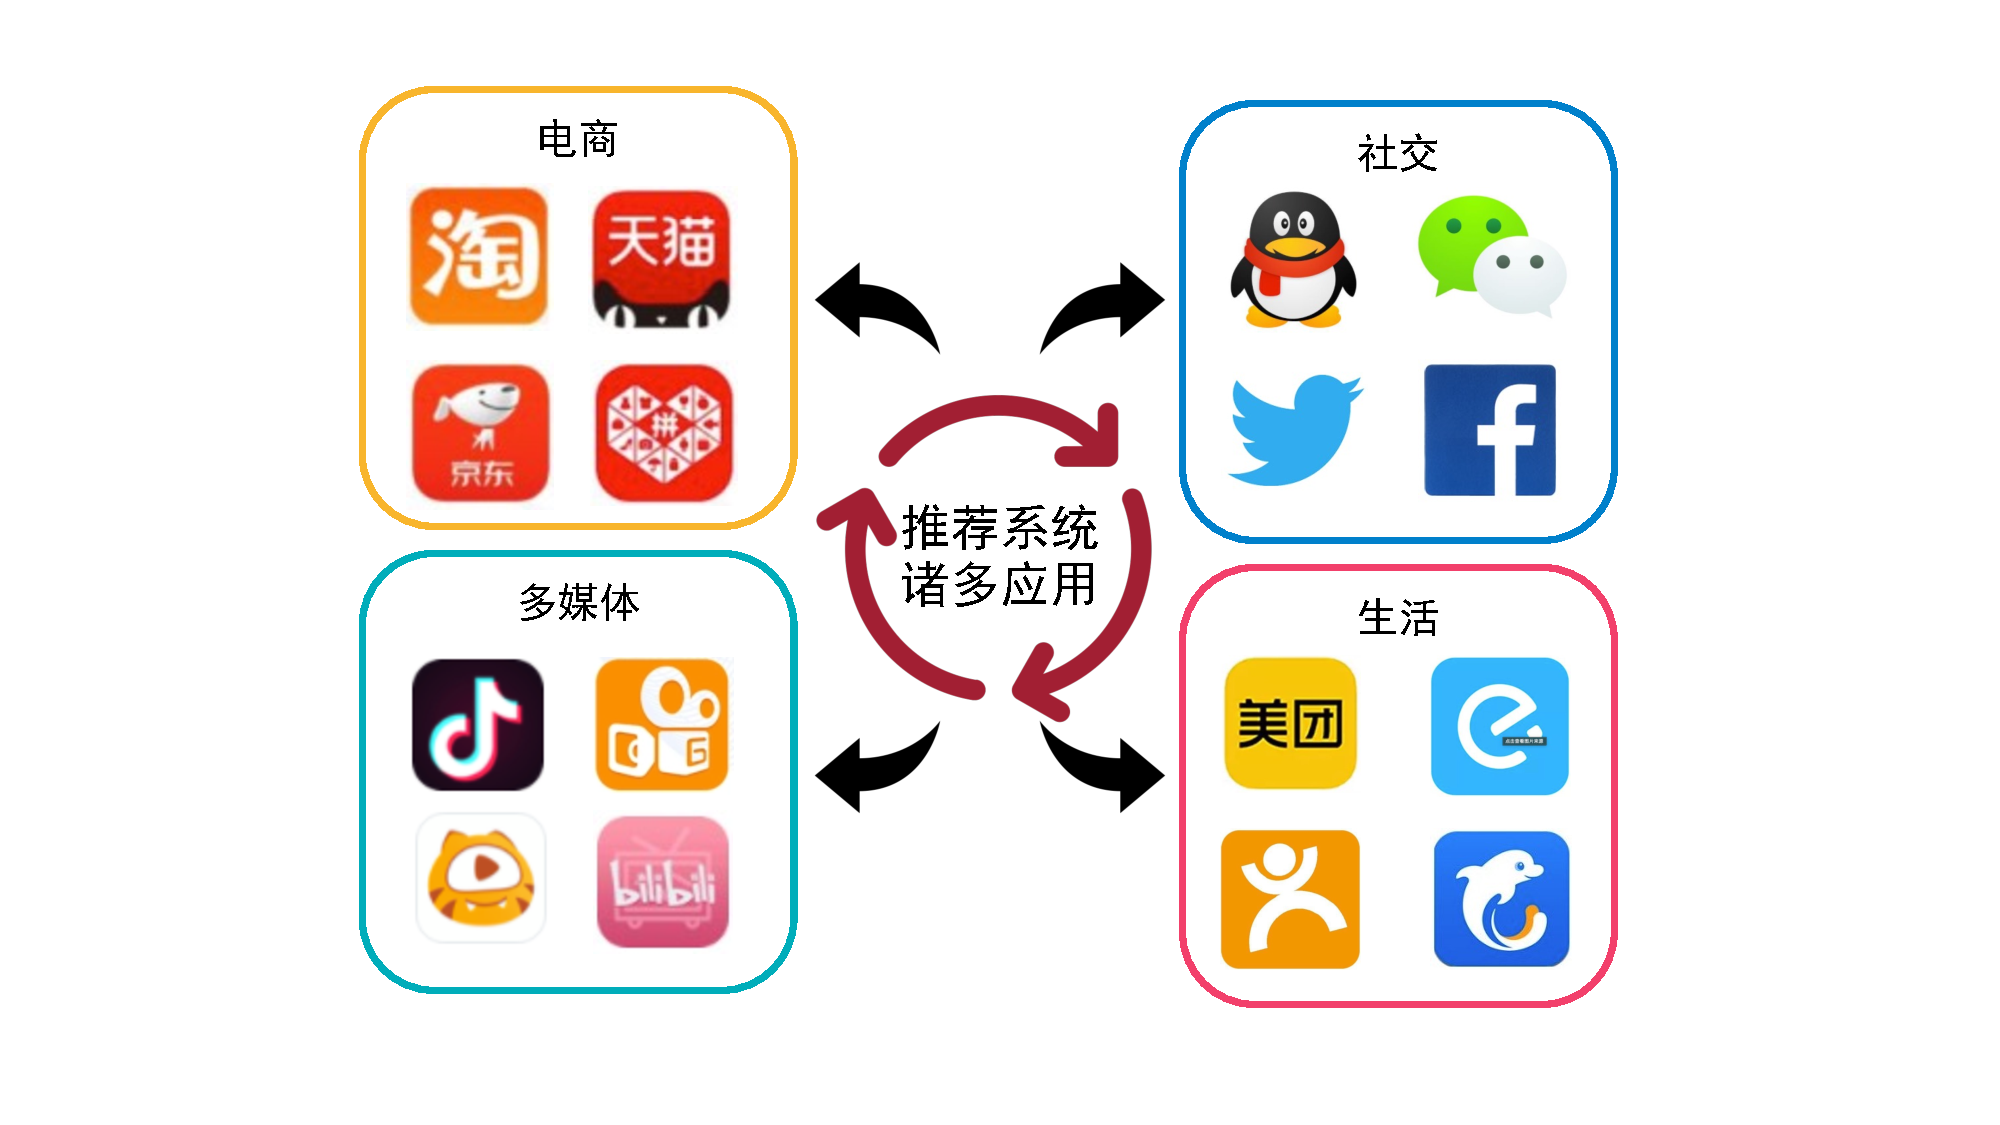
\includegraphics[width=0.6\linewidth]{figures/Introduction/apps.pdf}
  \caption{推荐系统的大量应用场景}
  \label{fig:apps}
\end{figure}

% 推荐系统的流程
随着深度神经网络技术的发展,向量化的推荐算法成为实际场景中广泛使用的算法\cite{su2020link, dhaware2020tourism, mukhopadhyay2008product}。向量化推荐系统将用户和物品编码成向量,在推荐过程中主要包括召回阶段和排序两大阶段,如图~\ref{fig:flowchart}所示。其中召回阶段负责从海量的数据中(百万-亿)初筛出一小部分数据(几十-百)用于后续的个性化推荐。排序阶段就是在召回阶段所筛选出数据的基础上,额外考虑用户的个性化信息,例如历史行为、用户画像等。最终将若干个结果推荐给用户。

\begin{figure}
  \centering
  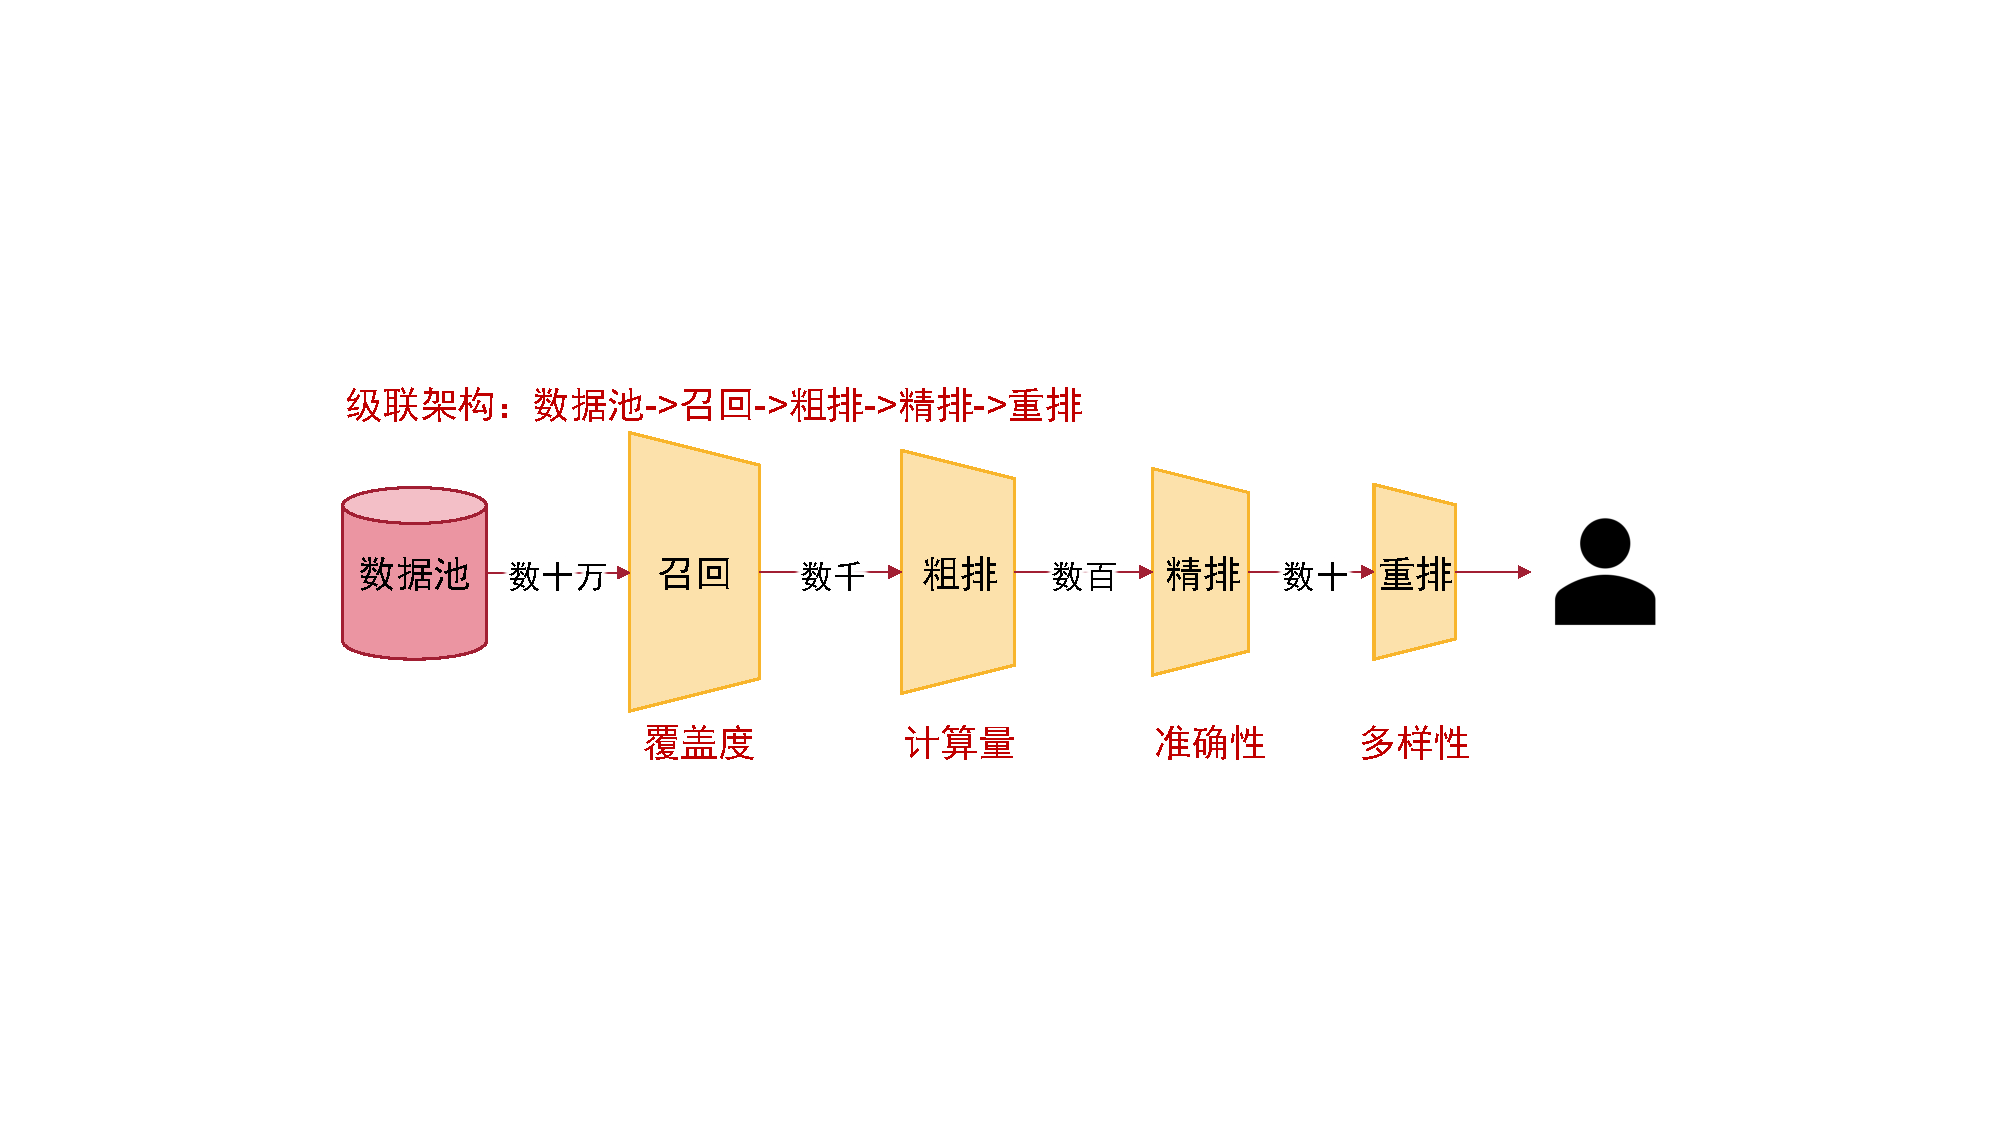
\includegraphics[width=0.9\linewidth]{figures/Introduction/flowchart.pdf}
  \caption{一般推荐系统流程图}
  \label{fig:flowchart}
\end{figure}

% 近似近邻搜索是推荐系统的核心组件
随着大数据时代的到来,近似近邻搜索成为推荐系统的核心组件\cite{chen2022approximate}。原因是推荐系统所需要处理的数据规模急剧增加,近似近邻搜索算法相比其他算法可以更快的完成对于大规模数据的高效处理\cite{wang2021comprehensive, jiang2020clustering, xu2022proximity}。如何进一步加速近似近邻搜索成为我们必须要面对和解决的问题。

% 基于图的近似近邻搜索目前被广泛使用由于其优越的性能
基于图的近似近邻搜索算法由于其优越的性能而被广泛使用\cite{chen2022finger, yu2022gpu, groh2022ggnn}。该算法将待搜索的向量看做高维空间中的点,通过一定的规则在这些点之间连接边,最后形成一张图。在线搜索的过程中,根据用户编码得到的查询向量,在图上进行搜索。
% 算法一般包括构建算法和搜索算法。构建算法就是在给定待搜索的数据集上构建图索引,搜索算法就是在图索引上根据给定的查询搜索与其最相似的结果。

% 基于图的近似近邻搜索存在构建和搜索方面的问题
随着大数据时代的到来,基于图的近似近邻搜索面临以下问题导致其性能难以支持海量数据下的推荐系统。首先,基于图的近似近邻搜索相比其他类型的算法需要更长的构建时间,随着新增数据量的增加,该方法面临严重的问题,可能导致图索引上的数据并不是最新,无法给用户准确的推荐物品。其次,现有硬件架构的低效导致基于图的近似近邻搜索在大规模数据的情况下,在推荐系统实时性的约束下,无法达到业务所需要的吞吐率。最后,现有基于图的近似近邻搜索的分布式算法的拓展性很差,考虑到单机的资源总是有限的,现有分布式算法的低效限制了其处理更大规模数据的潜力。

\section{研究现状}

近邻搜索(Nearest Neighbor Search,NNS)是在给定集合中找到与给定点最接近(或最相似)的点的优化问题\cite{nns-wiki}。精确求解这一问题只能采用暴力检索的方式,在大规模问题中难以应用。因此,研究者转向近似近邻搜索(Approximate Nearest Neighbor Search,ANNS),通过一定程度下可接受的精度损失,换取检索时间的极大降低。近似近邻搜索的核心思想就是将数据在某个维度的空间中做切分,减少需要遍历的数据量。根据空间划分方式的不同,大致可以分为以下四类:基于量化\cite{pq-2010, opq-2013, douze2016polysemous, zhang2019grip, kalantidis2014locally, abdelhadi2019accelerated}、基于树结构\cite{kdtree-2008, Annoy, houle2014rank,arora2018hd, muja2014scalable, wang2013trinary}、基于哈希(Locality-sensitive Hashing,LSH)\cite{lsh-1999, lsh-2004, sh-2008, sun2014srs, terasawa2007spherical, liu2014sk}和基于图结构\cite{kgraph-2011, nsw-2014, hnsw-2018, nsg-2019, dpg-2019}方法。如图~\ref{fig:ganns-vs-other}所示,由于实际数据的维度灾难等问题,基于图结构的近似近邻搜索方法取得了优于其余方法的效果,因此成为近年来的研究热点。本节将重点介绍基于图的近似近邻搜索方法的研究现状,同时也会对其余类型的方法做简要介绍。

\begin{figure}
  \centering
  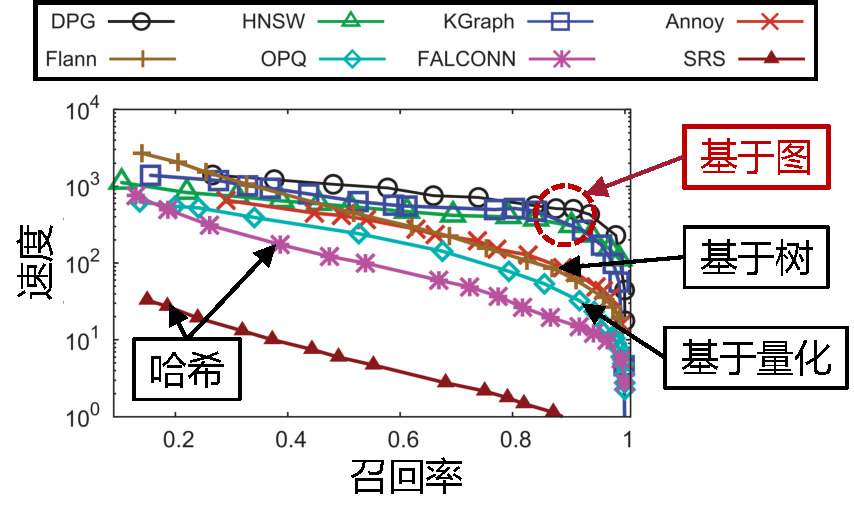
\includegraphics[width=0.7\linewidth]{figures/Introduction/ganns-vs-other.pdf}
  \caption{不同类型的近似近邻搜索方法的比较\cite{dpg-2019}(右上更好)}
  \label{fig:ganns-vs-other}
\end{figure}


\subsection{非图的近似近邻搜索方法}
非图的近似近邻搜索方法在构建开销和索引开销方面相比图方法具有一定的优势,因此在某些小数据集、存储资源匮乏的场景下也会被使用。非图的近似近邻搜索方法主要包括以下三类:
\begin{itemize}
  \item 基于量化的近似近邻搜索。这种方法通过量化编码的方式来近似表示原始数据空间。量化编码的好处一方面可以降低计算复杂度,另一方面也可以降低数据存储开销,但是量化会引入一定的近似导致最终搜索结果的准确性不足。
  其中的代表性方法包括:乘积量化\cite{pq-2010}(Product Quantization,PQ)是最具代表性的方法,它将数据在维度上切分为若干个子空间,然后使用每个子空间内的聚类中心点作为该类的编码。计算时只需要计算查询和这些编码的距离,将向量距离计算转换为查表操作。优化乘积量化\cite{opq-2013}(Optimized Product Quantization,OPQ)是在乘积量化的基础上,通过预处理的方式降低量化引入的误差。

  \item 基于树的近似近邻搜索。这种方法通过树结构的方式对数据空间进行划分,进而实现减少搜索时计算量的目的。该方法一般用于数据维度较低的场景中,一旦数据维度变高,该类方法的搜索效率将会显著降低\cite{AQA-1998}。
  其中代表性方法包括:K-D树\cite{kdtree-2008}(K-Dimensional Tree),K-D树通过所有的非叶子结点将数据空间逐级切分,每个叶子结点都代表一个多维数据。Annoy\cite{Annoy}(Approximate Nearest Neighbors Oh Yeah)以垂直平分两个聚类中心点连线的超平面将数据空间切分,然后通过递归的方式减少空间中的数据数量。

  \item 基于哈希的近似近邻搜索。这种方法是通过设计哈希函数将原始数据映射为哈希数据,进而降低计算的复杂度,同时还可以起到压缩数据的作用,但是哈希函数不可避免的会导致数据的信息损失进而影响精度。
  其中的代表性方法包括:局部敏感哈希\cite{lsh-1999,lsh-2004}(Locality-Sensitive Hashing,LSH)的核心思想是数据之间越相似,那么它们产生哈希冲突的概率也就越高。因此通过哈希函数后落入同一个哈希桶内的数据之间的相似概率更高,但是该方法还存在负载不均衡等问题。谱哈希\cite{sh-2008}(Spectral Hashing,SH)相比局部敏感哈希利用了数据空间的分布特性,可以从数据中学习哈希函数实现更优的映射。
\end{itemize}


\subsection{\ganns}
\ganns 方法将有限集合中的向量映射成高维空间中的点,核心思想是通过点之间的连接关系减少待搜索的空间。在构建阶段,通过一定的规则在这些点之间建立连接,这些点和边所组成的结构我们称之为图索引。在搜索阶段,对于用户给定的查询,在图上检索与查询最相似的若干个结果。我们从图索引上的某个点(搜索起始点)开始,迭代地搜索沿着这些边更接近查询的点。构建过程是连接这些点之间的边。不同的\ganns 方法之间的主要区别在于构建过程中使用的算法。

% TODO总结一下核心思想
\citet{hnsw-2018}等人提出的分层导航小世界图(Hierarchical Navigable Small World graphs, HNSW)是一种典型的\ganns 方法。相比之前的导航小世界图\cite{nsw-2014}(Navigable Small World graph,NSW)方法主要有两方面的改进,首先是层次化,HNSW由多个NSW图层组成;其次是选边策略,HNSW采用的是基于相对邻域图\cite{rng-1980}(Relative Neighbourhood Graph,RNG)的策略,该策略可以筛选出更加分布更加离散的邻居分布。在构建过程中,基向量中的每个点逐个添加到图索引中。每个点所在的最高层由一个概率指数衰减的随机函数决定,然后这个点需要添加到最高处以下的所有层中。然后,最底层包含数据空间中的所有点。

% TODO:Check 括号格式
\citet{nsg-2019}等人提出了导航扩展图(Navigating Spreading-out Graph,NSG),为预先构建的\textit{k-}近邻图(\textit{k-}Nearest Neighbor Graph,\textit{k-}NNG)上的每个点重新选择邻居。基于单调相对邻域图(Monotonic Relative Neighborhood Graph,MRNG)\cite{nsg-2019}的邻居选择策略保证每一步都比前一步更接近查询,但会导致过度的构建复杂度。因此,NSG采用近似的MRNG策略,将中心点确定为搜索起始点,减少构建复杂度。但NSG很难实现增量方式的构建,因为它需要预先构建好\textit{k-}近邻图。

多样化邻近图(DPG) \cite{dpg-2019}是在KGraph \cite{kgraph-2011}的基础上进行优化。其方法是对现有的k-近邻($k$-NN)图进行多样化,并添加反向边以提高搜索性能。对于数据点$p$,我们假设在$p$的近邻列表${L_N}$中有两个点$a$和$b$。然后定义角度$\theta (a,b) = \angle apb$。DPG使用贪婪启发式算法从${L_N}$中选择一个子集$S$,以最大化$S$中两点之间的平均夹角。此外,DPG设置图中某个点的最大连通邻居数(即$k$),以找到$k$ NN图的多样性和邻近性之间的良好权衡。

% \subsection{\ganns 的硬件工作}
% diskann spann ggnn


\section{研究内容与主要贡献}

\begin{figure}
  \centering
  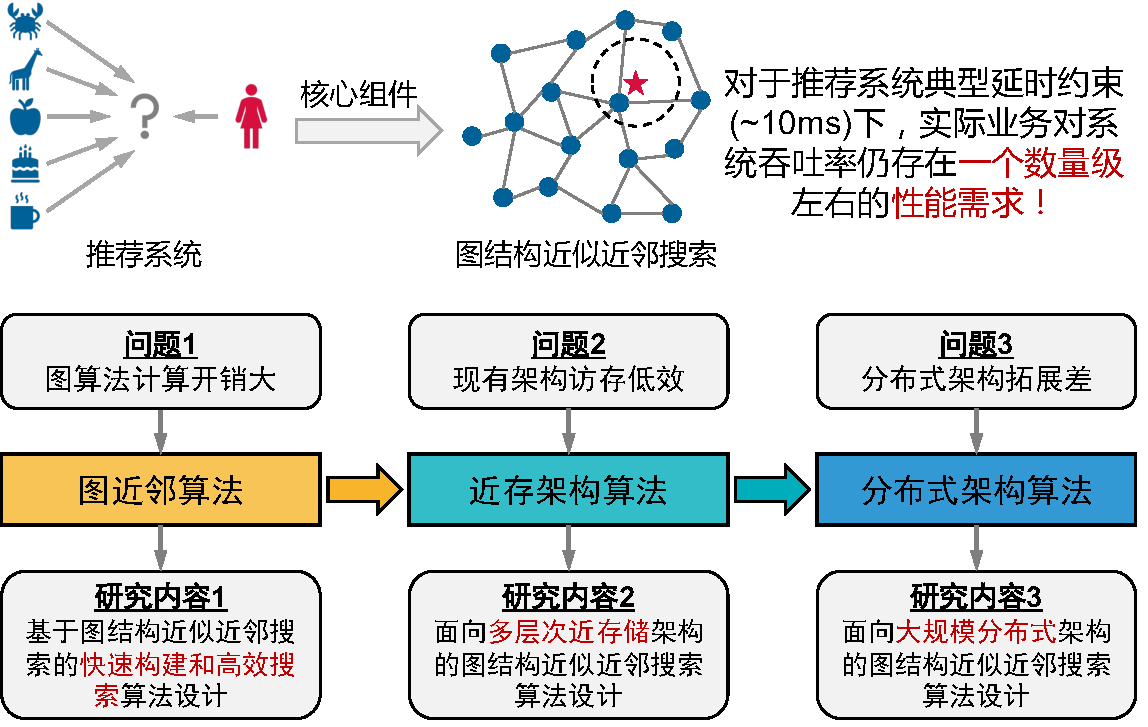
\includegraphics[width=0.7\linewidth]{figures/Introduction/overview.pdf}
  \caption{本文的整体研究内容}
  \label{fig:overview}
\end{figure}

% 数据检索中图方法很好,但是在大数据时代下面临挑战
综上所述,尽管基于图的方法相比其他类型的近似近邻搜索方法在以推荐系统为代表的数据检索问题中表现出更优的性能,但其仍然存在的三个问题限制了在大数据时代下的应用潜力。
首先,\ganns 方法相比其他方法具有更长的构建时间\cite{dpg-2019},其原因是在构建阶段的计算开销大。因此在海量数据下难以做到对新增数据的及时更新,进而影响推荐系统的服务质量。其次,\ganns 方法在现有硬件架构上运行效率低下,其原因是\ganns 在计算过程中涉及大量的数据搬运,进而在冯诺依曼这种存算分离的架构上表现低效。以CPU为例,整个执行过程的80\%以上开销在访存,这一问题在大规模数据下会更为严重。最后,随着数据规模的不断增加,单机的处理能力总是有限的,而现有针对多机的\ganns 方法存在拓展性差的问题。总的来说,\ganns 的这些问题限制了在大数据时代下的应用潜力,以推荐系统这一典型场景为例,仍然存在一个数量级以上的性能差距。

% TODO:替换“我们”这种表述
图~\ref{fig:overview}给出了本文的整体研究内容,本文主要从构建算法、近存算法和多机算法三个方面开展研究设计,分别针对上述问题提出解决方案。其中后两个研究内容主要是针对搜索算法的,因为在实际中搜索算法是在线进行的。
针对第一个问题,本文研究高效的构建算法设计,以降低构建阶段的计算开销。\todo{具体解法是什么?}

针对第二个问题,本文研究面向近存架构的高效算法设计,结合不同层级的近存架构特点设计相应的算法,充分发挥近存架构的潜力。首先本文对\ganns 的搜索算法所设计的算子进行抽象和分析,建立了硬件分析模型。然后基于硬件分析模型,对近内存处理架构提出了并行方案的设计。最后考虑到大规模数据下的情况,拓展了近外存处理架构,并结合外存的访存特点对算法进行了流水设计。

针对第三个问题,本文研究面向多机分布式的高效算法设计,有效提高了\ganns 方法的拓展性。首先本文在现有多机方法的基础上提出了一套通用的多机并行框架,并分析了现有无通信方式在图结构下的不足和问题。然后针对多机并行框架具有更高理论上限的全图方式,在直接的方案下会严重受限于通信开销这一问题,分别提出了索引预先加载策略和特征延迟处理策略,大幅减少了通信开销,有效提升了\ganns 方法在大规模数据下的拓展性。

% \begin{figure}
%   \centering
%   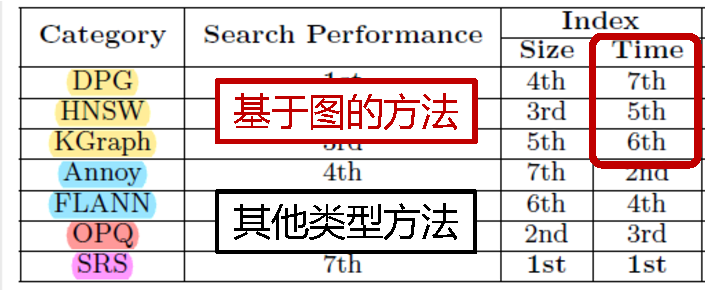
\includegraphics[width=0.6\linewidth]{figures/Introduction/ganns-index.pdf}
%   \caption{基于图的近似近邻搜索方法需要更长的构建时间\cite{dpg-2019}}
%   \label{fig:ganns-index}
% \end{figure}



\section{本文的组织结构}
本文的组织结构如下:

首先,本文在第1章中详细阐述了本文的研究背景和意义,并介绍了相关工作的研究现状,指出\ganns 方法所面临的问题和优化机会,并在最后简要总结了本文的主要贡献和研究内容。

第2章介绍相关研究的基础知识。首先介绍了\ganns 的问题定义、构建过程和搜索过程,然后介绍了近存架构的概述。

第3章针对\ganns 中构建阶段的计算开销大的问题,研究构建算法的设计。\todo{内容}

第4章和第5章重点考虑\ganns 的搜索阶段的加速。第4章针对\ganns 在现有硬件架构上面临执行能效低下的问题,研究高效的近存算法设计。

第5章针对\ganns 拓展性差,难以处理更大规模数据的问题,研究高效的多机算法设计。

最后,第6章总结了本文的核心思路和主要创新点。并提出了本文工作在未来可能的研究方向。
% !TeX root = ../main.tex
\renewcommand{\algorithmicrequire}{\textbf{输入:}\unskip}
\renewcommand{\algorithmicensure}{\textbf{输出:}\unskip}

\chapter{基于图近似近邻搜索的研究基础}
上一章节针对本文拟开展研究的背景和意义进行了简要说明和讨论。本章节承上启下,对上所述的研究背景进一步展开叙述,对下所开展研究的基础进行了详细介绍。首先在\ref{sec:bg-anns}节中介绍近似近邻搜索问题的定义和评价指标。然后在\ref{sec:bg-ganns}节中以\ganns 方法中最典型的HNSW算法为例,详细介绍其构建过程和搜索过程。最后在\ref{sec:bg-rm}节中,本文以近似近邻搜索方法的典型应用场景——推荐系统为例,简要介绍推荐系统的整体流程以及本文所研究的近似近邻搜索方法在其中的应用。


\section{近似近邻搜索问题}\label{sec:bg-anns}
近邻搜索问题是一个由来已久的经典问题,本节首先给出近邻搜索和近似近邻搜索的问题定义,明确本文的研究问题。由于近似方法会引入一定的精度损失,因此紧接着本文会介绍在近似近邻搜索问题中的几个重要指标,最后介绍常见的几种相似度度量方式。

\subsection{问题定义}
\textit{最近邻搜索(Nearest Neighbor Search, NNS)}是一个优化问题,其目标是在给定的有限集合$X \subset \mathbb{R}^d $中寻找与给定查询$q \in \mathbb{R}^d$最相似的结果。这一问题可以被表示为:
\begin{equation}
R = \mathop{\arg\min}\limits_{x \in X} dist \left\langle q,x \right\rangle 
\label{eq:nns}
\end{equation}

其中,$X$是底库数据集,$dist \left \langle q,x \right \rangle$是距离度量(例如,欧式距离或内积距离等),以表示$q$和$x$之间的相似性。类似地,我们还进一步拓展到\textit{k-近邻搜索(k-Nearest Neighbor Search)},寻找最相似的\textit{k}个结果,也就是将式\ref{eq:nns}中的$R$表示为$R_k$。

不幸的是,随着底库数据集$X$中数量以及数据维度的增加,精确的近邻搜索任务采用穷举式方法,搜索时间变得不可接受。因此,研究人员将研究重心转向了近似方法,即\textit{近似近邻搜索(Approximate Nearest Neighbor Search, ANNS)},这种近似方法通过精度的略微下降,换取搜索时间的大幅降低。总的来说,近似近邻搜索方法的核心思想都是借助一定的已知信息,减少在搜索过程中需要计算相似度的数据数量。典型的利用已知信息构建索引的方法包括基于树、基于图、基于量化、基于哈希等多种方法。

\subsection{评价指标}
\begin{itemize}
    \item 精度: 搜索精度通常用召回率(Recall Rate)来表示,本文中有时也用准确率表示。对于某个查询$q$,通过近似近邻搜索方法找到它的$k$个结果表示为$R_{k}'$。实际的前$k$个最相似的结果为$R_k$,那么召回率$Recall@k$(简称:$R@k$)的定义如下:
    \begin{equation}
    Recall@k = \frac{{\left| {R_{k}' \cap R_{k}} \right|}}{{\left| {R_{k}} \right|}} \label{eq:recall}
    \end{equation}
    
    \item 性能:搜索性能通常由吞吐率(Throughout)和延时(Latency)来表示。其中吞吐率的单位一般是每秒查询数(Query-Per-Second, QPS),它用来衡量单位时间内可以完成的查询数量,越大越好。延时以时间单位作为测量,例如毫秒,它用来衡量系统的响应时间,越低越好。然而对于给定的算法和系统,更高的吞吐率和更低的延时之间是矛盾的,需要根据具体任务做权衡(Trade-off)。
\end{itemize}

一般来说,上述三种评价指标均指针对一个查询集合的测量,而不是仅仅测量系统执行一次查询任务的结果。对于QPS,我们一般用查询集合中查询数据的数量除以所有查询数据被系统处理完成的总时间来表征。对于召回率和延时,我们一般对每一个查询数据进行单独的评估,并最终进行平均来表征。

\subsection{相似度度量方式}
在近邻搜索问题中,两个数据之间相似程度的一般采用这两个$d$维向量之间的距离表示。近似近邻搜索问题中常用的距离计算方式有三种:欧氏距离\cite{dokmanic2015euclidean},内积距离\cite{critchley1988certain}和余弦距离\cite{zou2008shape, nguyen2010cosine}。

接下来,我们以向量$\overrightarrow a~({a_1},{a_2}, \cdots ,{a_N})$和向量$\overrightarrow b~({b_1},{b_2}, \cdots ,{b_N})$为例介绍上述三种距离度量方法。向量$\overrightarrow a $与$\overrightarrow b $之间的距离记为$d(\overrightarrow a ,\overrightarrow b )$。
\begin{itemize}
    \item 欧氏距离:在数字图像处理中有着广泛的应用。其计算公式如下:
    
    \begin{equation}
    d(\overrightarrow a ,\overrightarrow b ) = \sqrt {\sum\limits_{i = 1}^N {{{({a_i} - {b_i})}^2}} } \label{eq_Eu}
    \end{equation}
    
    \item 内积距离:它是在内积空间中定义的,这使得我们可以讨论向量的角度和长度。其计算公式如下:
    
    \begin{equation}
    d(\overrightarrow a ,\overrightarrow b ) = {\sum\limits_{i = 1}^N {{a_i}{b_i}} }\label{eq_ip}
    \end{equation}
    
    \item 余弦距离:更多的是从方向上区分差异,对绝对值不敏感。余弦距离由余弦相似度$\cos (\overrightarrow a ,\overrightarrow b )$转换而来,如\eqref{eq_cos1}和\eqref{eq_cos2}所示。
    
    \begin{equation}
   \cos (\overrightarrow a ,\overrightarrow b ) = \frac{{\sum\limits_{i = 1}^N {{a_i}{b_i}} }}{{\sqrt {\sum\limits_{j = 1}^N {{a_i}^2} } \sqrt {\sum\limits_{k = 1}^N {{b_i}^2} } }}\label{eq_cos1}
    \end{equation}
    
     \begin{equation}
    d(\overrightarrow a ,\overrightarrow b ) = 1 - \cos (\overrightarrow a ,\overrightarrow b )\label{eq_cos2}
    \end{equation}
\end{itemize}



\section{\ganns}\label{sec:bg-ganns}
如前所述,\ganns 方法相比其他类型的近似近邻搜索方法有更好的性能而被广泛使用。如图~\ref{fig:ganns}所示,\ganns 方法由构建和搜索两个过程组成,其中构建过程根据给定的数据集生成其中数据点之间的连接,被称为图索引,这个过程一般是离线进行的。搜索过程是基于构建好的图索引,在其上对给定的查询进行查找,并给出最终最相似的若干个结果,这个过程一般是在线进行的,也是实际应用中大家关注的重点。本节基于其中最具有代表性的\textit{分层导航小世界图(Hierarchical Navigable Small World graphs, HNSW)\cite{hnsw-2018}}算法,作为例子详细介绍其构建过程和搜索过程。需要注意的是,\ganns 方法之间的搜索算法基本上是相同的,主要区别在于构建过程。因此本节关于搜索过程的介绍也可以容易拓展到其他的\ganns 方法上。

\begin{figure}
  \centering
  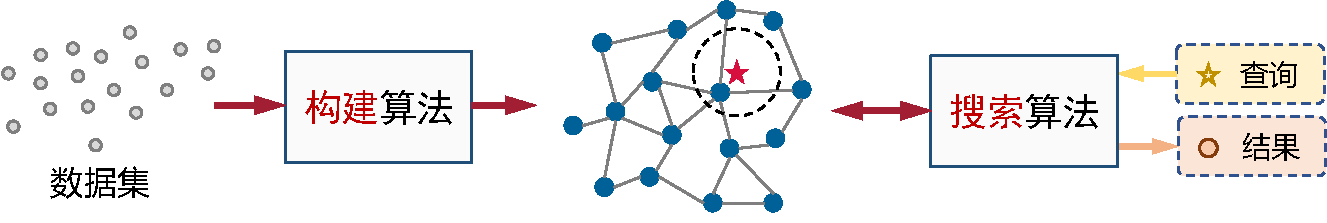
\includegraphics[width=0.9\linewidth]{figures/Background/ganns.pdf}
  \caption{\ganns 方法的整体流程}
  \label{fig:ganns}
\end{figure}

% TODO:这块的逻辑怎么加?
% 对于基于图的ann算法,我们用图上的点和边来表示基向量之间的关系。因此在下文中,我们将$i$-th的基向量和它的连接分别称为$i$-th点的特征和邻居列表。

\subsection{构建过程}
近似近邻搜索方法的构建过程就是根据一定的构建算法将底库数据集中的点之间连接起来。HNSW所采用构建算法的主要特点有两个,一是层次图结构,二是基于相对邻域图\cite{rng-1980}(Relative Neighbourhood Graph,RNG)的邻居选择策略。其中层次图结构在\todo{XX}中被证明仅在数据维度较低的情况下有效,对于高维数据无法起到加速搜索的效果,但本文基于完整性的考虑仍然会进行介绍。


HNSW采用增量式的构建算法,即底库数据集中的数据是逐个添加到图结构上。不失一般性的,本文针对其中某个点的添加过程进行详细阐述,相应的伪代码如算法~\ref{alg:construct}所示。假设当前图索引的最高层为$l_{max}$(从0开始编号)。
\begin{enumerate}
    \item 首先,通过一个随机函数得到该待添加点最高所在的层$l_c$,这个随机函数是一个负对数函数,可以保证最底层(即第0层)图中包含数据集中所有的数据点,而随着层编号的增加,对应层的数据点数呈固定倍数下降(eg.$M$,第0层外的其他层图中的最大邻居数),且每一层(除第0层)的数据点集合均为其下一层数据点集合的子集。
    \item \textbf{迭代更近的起始点}。我们将待添加的点视为一个查询点,在现有的图索引结构中,从最高层$l_{max}$开始逐层向下搜索,一直到第$l_c+1$层,在每一层图上搜索与它最近的点,并将这个最近的点作为下一层搜索时的起始点。
    \item \textbf{将点添加到图索引上}。我们需要在图索引的第$l_c$层到第0层中的每一层上插入待添加的数据点。具体流程分为以下三个步骤: 
    \begin{enumerate}
        \item 候选点搜索。将待添加点视为一个查询点,并在当前层的索引中搜索与它最近的$efc$个点作为候选点。
        \item 邻居选择。从上述在索引中找到的$efc$个点中,通过某种邻居选择策略,选出不超过$M$个点,作为该点的邻居点。对于HNSW算法,采用的邻居选择策略如算法~\ref{alg:RNG}所示。
        \item 邻居反向选择。对上述的邻居点,需要将该待添加点添加为这些邻居点的邻居。在这个过程中,一旦某个点的邻居数超过最大邻居数$M$,则需要使用上述的邻居选择策略进行筛选,以保证所有点的邻居数量始终不超过$M$。
    \end{enumerate}
\end{enumerate}


\begin{algorithm}
    \caption{HNSW构建算法}
    \label{alg:construct} 
    \begin{algorithmic}[1]
        \REQUIRE
        底库数据集 $X$, 最大邻居数 $maxM0$, 起始点 $p_s$
        \ENSURE
        图索引 $G_N$
        \FOR{$p_{in} \in X$}
        \STATE $Q_{cand}^{in} \gets$ greedy search$(q,G_s,p_s,efc,efc)$
        \STATE $Q_{sel}^{in} \gets$ SelectNeighborByRNG$(p_{in},Q_{cand}^{in},maxM0)$
        \STATE $Neighbor(p_{in}) \gets Q_{sel}^{in}$
        
        \FOR{$p_r \in Neighbor(p_{in})$}
        \STATE $addNeighbor(pr) \gets p_{in}$
        \ENDFOR
        \ENDFOR
        \RETURN $G_N$
    \end{algorithmic} 
\end{algorithm}

\begin{algorithm}
    \caption{基于RNG的邻居选择策略 SelectNeighborByRNG($p_c,S_{cand},maxM0$)}
    \label{alg:RNG}
    \begin{algorithmic}[1]
        \REQUIRE
        点 $p_c$, 候选集合 $S_{cand}$, 最大邻居数 $maxM0$.
        \ENSURE
        选出的邻居集合 $S_{sel}$.
        \STATE $S_{sel} \gets \emptyset$
        \FOR{$x_i \in S_{cand}$}
        \IF{$S_{sel}.size = maxM0$}
        \STATE \textbf{break}
        \ENDIF
        
        \STATE $dist \gets getDistance(p_c, x_i)$
        \FOR{$s_i \in S_{sel}$}
        \STATE $d \gets getDistance(x_i, s_i)$
        \IF{all $d>dist$}
        \STATE $S_{sel} \gets S_{sel} \cup x_i$
        \ELSE
        \STATE \textbf{break}
        \ENDIF
        \ENDFOR
        \ENDFOR
        \RETURN $S_{sel}$
    \end{algorithmic} 
\end{algorithm}

接下来进一步介绍HNSW算法中采用的邻居选择策略。简单连接策略将最近的点连接到$p_c$,如图~\ref{fig:nbor-select-a}所示,这显然会导致局部密度的问题。因此,HNSW采用基于RNG的连接策略。与简单连接策略相比,基于rng的邻居选择策略改善了这一缺点,使节点的邻居更加分布在整个空间中,避免了大量节点的邻居集中在某一区域。RNG的具体方法如下图~\ref{fig:nbor-select-b}所示。从一个排序好的待连接的节点队列中,依次取出距离最小的点,然后找到一种方法来判断是否将该点加入邻居。具体方法如图所示。假设$x$是点$p_c$的邻居,对于要连接的某个点$q$,对于任何满足关系$dist(q,x)>dist(x,p_c)$的$x$, $q$被添加为$p_c$的邻居,并继续循环,直到队列中没有要连接的元素或邻居数量达到最大值。RNG策略递归比较当前待连接点与现有邻居之间的距离关系,以确定当前待连接点是否会成为邻居。因此,基于RNG的节点连接策略使节点的邻居均匀分布在空间中,避免了部分邻居过度集中而降低搜索性能。总结来说,尽管基于RNG的邻居选择策略相比简单连接策略可以一定程度上避免陷入局部最优,但是也引入了更多的计算开销。

\begin{figure}
  \centering
  \subcaptionbox{直接选择策略 \label{fig:nbor-select-a}}
    {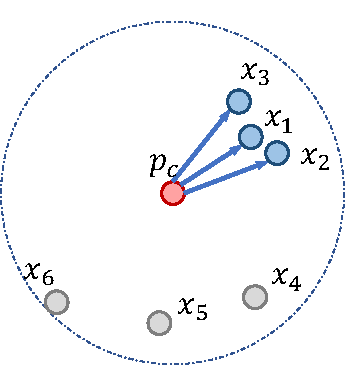
\includegraphics[width=0.35\linewidth]{figures/Background/select-naive.pdf}}
  \subcaptionbox{RNG选择策略 \label{fig:nbor-select-b}}
    {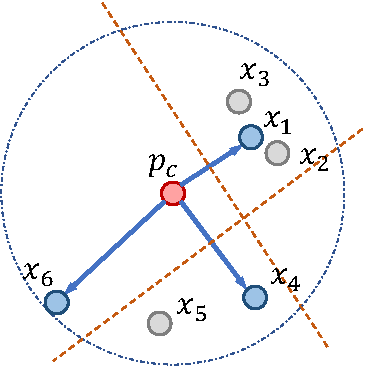
\includegraphics[width=0.35\linewidth]{figures/Background/select-rng.pdf}}
  \caption{两种近邻选择策略在二维空间中的直观对比。(a)直接连接策略只选择距离较近的点作为邻居,而(b)RNG连接策略尽可能挑选在空间中分散的点作为邻居。}
  \label{fig:nbor-select}
\end{figure}



\subsection{搜索过程}

绝大多数\ganns 方法的搜索过程都采用最佳优先搜索\cite{nsg-2019, ganns-survey-2021}(Best First Search)算法(以及其变种)。对于HNSW算法而言,在第0层图上搜索与查询最近的$k$个结果,在其余层图上搜索与查询点最近的一个点作为下一层图的搜索起始点。因此,本文在本节会详细介绍最佳优先搜索算法在单层图上的实现方式,其伪代码如算法~\ref{alg:search}所示。

HNSW所使用的最佳优先搜索算法是一种迭代式的算法,每轮迭代都不断地选取与查询点更近的点进行下一轮迭代。搜索过程中,我们需要维护三个集合:待搜索队列、结果队列、已搜索集合。其中待搜索队列和结果队列均为优先队列,其中元素按照与查询点的距离排序,距离越近的元素越排在队列的前面。
对于每次迭代,我们首先从待搜索队列中选择最接近查询点的位于队列首的点作为搜索点。然后,从该搜索点的邻居列表中读取所有邻居,并通过已搜索集合对其进行过滤,以避免重复的计算操作。接下来,计算查询点与这些邻居之间的距离。最后将距离和邻居信息插入两个优先队列以及已搜索集合。这个过程重复进行$ef$轮迭代后,我们从结果队列中读取查询的topK结果。这里$ef$是一个控制精度-速度权衡的超参数。


\begin{algorithm}[t]
  \caption{最佳优先搜索算法 Search ($q, G, p_s, efs, k$)}
  \begin{algorithmic}[1]
    \REQUIRE 
    查询点 $q$, 图索引 $G$, 起始点 $p_s$, 控制精度-速度权衡的超参数 $efs$, 目标结果数量 $k$
    \ENSURE
    距离 $q$ 最近的 $k$ 个点
    \label{alg:search}
    \STATE $Q_r \gets p_s$ $//$结果队列 (队首距离查询点最近)
    \STATE $Q_{sn} \gets p_s$ $//$待搜索队列 (队首距离查询点最近)
    \STATE $bound \gets getDistance(q,p_s)$
    \WHILE{$Q_{sn}.size>0$}
      \STATE $p_f \gets Q_{sn}.top$
      \STATE $Q_{sn}.pop$
      \IF{$getDistance(q,p_f)>bound$}
        \STATE \textbf{break}
      \ENDIF
      \FOR{$p_n \in Neighbor(p_f)$}
        \STATE $d \gets getDistance(q,p_n)$
        \IF{$d<bound$ || $Q_r.size<efs$}
          \STATE $Q_{sn} \gets Q_{sn} \cup p_n$
          \STATE $Q_r \gets Q_r \cup p_n$
          \IF{$Q_r.size>efs$}
            \STATE $Q_r.pop$
          \ENDIF
          \STATE $bound \gets getDistance(q,Q_r.top)$
        \ENDIF
      \ENDFOR
    \ENDWHILE
    
    \WHILE{$Q_r.size>k$}
    \STATE $Q_r.pop$
    \ENDWHILE
    \RETURN $Q_r$
  \end{algorithmic} 
\end{algorithm}


接下来,本文以一个例子来演示上述的搜索算法。在图\ref{fig:search-step}中按顺序展示了在图上的前三个步骤的搜索过程。在搜索过程开始时,搜索队列$Q_{sn}$中只有起始搜索点$p_s$。对于搜索过程的每个\textbf{步骤},我们从搜索队列中弹出最接近查询(五角星)的点作为当前搜索点$p_f$(红色)。然后我们计算当前搜索点的所有邻居与查询之间的距离,并将这些邻居添加到待搜索队列和结果队列$Q_r$。待搜索队列由所有绿色点组成,而结果队列保存了非灰色点(绿色、红色和紫色)中最接近查询点的$efs$个点。紫色的点表示上一步的当前搜索点。然后执行下一步,直到满足终止条件。最后,在结果队列$Q_r$中与查询最近的$k$点用作搜索结果。

\begin{figure}
  \centering
  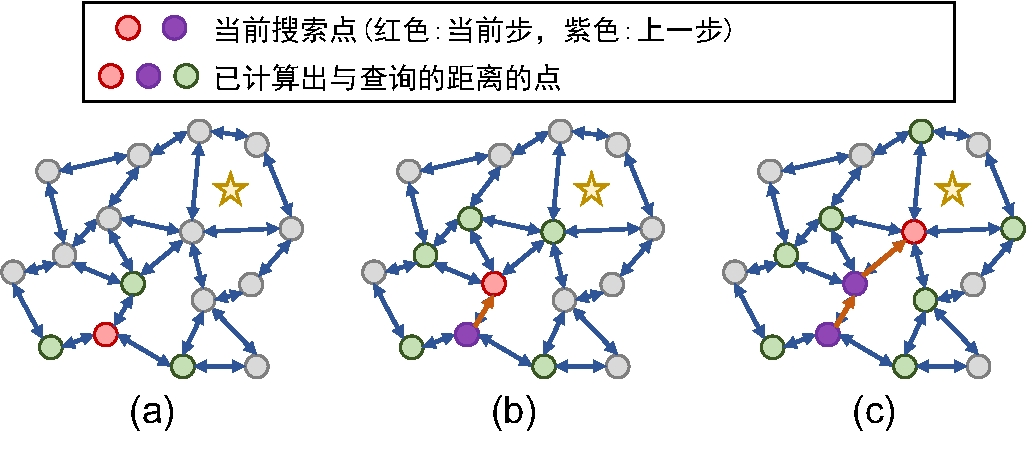
\includegraphics[width=0.8\textwidth]{figures/Background/search-step.pdf}
  \caption{在图索引上搜索查询最近邻的示意图。(a)-(c)分别表示搜索过程的前三步。}
  \label{fig:search-step}
\end{figure}


NSG虽然也采用迭代的方式,但数据结构有所不同,它仅维护一个待搜索集合。对于每次迭代,首先从待搜索集合中选择最接近查询点的未被标记为已搜索的点作为搜索点,并将该搜索点标记为已搜索。然后,从该搜索点的邻居列表中读取所有邻居,并通过待搜索集合对其进行过滤,以避免重复的计算操作。接下来,计算查询点与这些邻居之间的距离后将距离和邻居信息插入待搜索集合。最后,将待搜索集合按照与查询点的距离进行排序,并限制集合的最大尺寸$l$。这个过程重复进行$l$轮迭代后,从结果队列中读取查询的topK结果。虽然NSG的搜索算法减少了集合数量,但导致每次决定搜索点时需要进行遍历以寻找未被标记为已搜索的点,一定程度上损失了一定的搜索性能。


% \begin{itemize}
%   \item 特征矩阵:其大小为$N \times D$,其中$N$表示基向量的数量,$D$表示基向量的维度。$i$ -th行表示$i$ -th点的基向量。
%   \item 邻居矩阵:其大小为$N \times \left( M+1 \right) $,其中$M$表示最大邻居数。$i$ -th行表示$i$ -th点的邻居列表(从第二列开始),实际的数字由第一列表示。
%   \item Queue:它是一个升序队列(根据$Dist.$),长度为$efs$(超参数),其中每个元素是$\left\{ Id, Dist., Flag \right\} $。$Dist.$表示$Id$ -th基向量和查询向量(query)之间的距离,$Flag$表示点的状态(True: unsearches, Flase: searches)。 
%   \item Visited Table:长度为$N$。$i$ -th位置的值表示是否计算了$i$ -th点到查询的距离。
% \end{itemize}

% 每个查询的搜索过程执行几个循环(步骤),步骤的数量与超参数$efs$正相关。搜索过程完成后,将使用队列中排名靠前的$k$$Id$作为查询结果。如图\ref{fig:search process}所示,$i$ -th步骤可以分为以下四个阶段(操作)。

% \begin{enumerate}
%   \item 选择。首先,我们需要选择\textit{搜索点}($p_s$)并将其$Flag$更改为False。如果是$i=1$,则搜索点是整个图的起点。否则,搜索点就是队列中最近的未搜索点。
%   \item 查找&过滤。我们根据搜索点在邻居矩阵上查找相应的邻居列表。然后,我们通过访问过的表对邻居列表进行过滤,以避免重复计算。 
%   \item 距离计算。根据近邻列表找到特征矩阵上对应的基向量,并逐个计算与查询向量的距离。
%   \item 排序。我们将上一阶段计算的$\left\{ Id, Dist., True \right\} $逐个插入到队列中。然后,如果队列中所有点的$Flag$ s都为False,则搜索过程结束。相反,$Flag$为真的点中$Dist.$最小的点是\textit{最近的未搜索点}。
% \end{enumerate}


\section{和推荐系统之间的关系}\label{sec:bg-rm}

以图结构算法为代表的近似近邻搜索方法广泛用于推荐系统中。在向量化推荐系统中,所有的物品和用户都可以被编码后的向量表示,这一阶段被称为嵌入(Embedding)\cite{yi2019deep, zhang2016collaborative, khoshneshin2010collaborative, chen2019collaborative, rahutomo2019embedding}。推荐系统一般可以被分为两个阶段:召回阶段和排序阶段。在召回阶段,系统需要从所有的物品或内容中,快速找到一些可能与用户感兴趣的物品或内容最相似的候选物品或内容,以减少后续的排序计算量。在排序阶段,系统则需要对召回的候选物品或内容进行精细的排序,以保证用户最可能感兴趣的物品或内容排在前面。
\begin{itemize}
  \item \textbf{召回阶段}~在召回阶段中,近似近邻搜索算法可以帮助推荐系统快速找到与用户感兴趣的物品或内容最相似的一些候选物品或内容。具体来说,近似近邻搜索算法可以对所有的物品或内容进行预处理,建立索引等数据结构,以快速地定位到与用户查询最相似的一些物品或内容。由于基于图的近似近邻搜索算法可以快速处理高维度的数据,因此在推荐系统中使用基于图结构的近似近邻搜索算法可以大大提高召回阶段的效率和准确率。
  \item \textbf{排序阶段}~在排序阶段中,通常使用一些机器学习或深度学习的方法,如逻辑回归\cite{wang2016mobile, oladipo2021improved, tian2019music}、神经网络\cite{liu2016recurrent, rivas2020social, covington2016deep}等,对召回的候选物品或内容进行排序。这些方法可以利用用户的历史行为、兴趣偏好等信息,对候选物品或内容进行打分,并将打分高的物品或内容排在前面。然而,如果召回阶段的候选物品或内容质量不高,即与用户感兴趣的物品或内容不够相似,那么排序阶段也很难得到良好的排序结果。因此,近似近邻搜索在推荐系统中的重要性就在于,它可以帮助推荐系统在召回阶段中找到高质量的候选物品或内容,从而提高排序阶段的效果。
\end{itemize}





% \section{近存储计算架构的概述}


% !TeX root = ../main.tex

\chapter{近邻图算法优化}
上一章中针对本文拟开展研究的基础进行了详细的阐述。本章立足于近邻图算法,首先在\ref{sec:galg-overview}节中指出现有\ganns 方法(以HNSW为代表)存在的问题和不足,分别是图连通性差和搜索过程存在冗余。然后在\ref{sec:galg-connection}节中针对图连通性差这一问题,进行分析并提出反向连接增强策略。在\ref{sec:galg-earlystop}节中针对搜索过程存在冗余这一问题,分析其原因并提出查询感知早停策略。


\section{概述}\label{sec:galg-overview}
尽管\ganns 方法相比其他类型的近似近邻搜索方法取得了成功,但其仍然存在诸多不足。首先,基于图的近似近邻搜索方法通常需要通过建立图来表示数据集。但是,当数据集的分布较为分散时,图的连通性可能会变得较差。这样的话,搜索算法就可能会错过一些真正接近查询点的近邻点。此外,在高维数据的情况下,基于图的近似近邻搜索方法也可能会遇到所谓的“维数灾难”问题,随着数据维数的增加,类似HNSW算法的多层图结构的效果变得越来越差,基本与单层图无异,因此本文中采用的都是单层图。其次,基于图的近似近邻搜索方法在搜索过程中还存在一些冗余。具体来说,由于它是基于图的方法,每个点都会与周围的一些点建立联系。然而,这些联系并不一定都是有意义的,有些联系甚至可能会干扰搜索算法的正常工作。

\subsection{图连通性差}
在\ganns 方法中,查询点根据图上点之间的连接,以迭代的方式查找它的相似点。因此,图索引的连通性对于最终的搜索结果至关重要。具体来说,某一点的入度越大,能找到它的点越多(搜索精度越高)。某个点的出度越大,每一步的搜索代价越大(搜索速度越慢)。一些入度较小的点的存在意味着图索引的连通性较差。对于某个查询点来说,如果这些入度较小的点属于查询点的真值,但在搜索过程中没有找到,则会导致较低的召回率。
本文通过实验来说明这一点,如图~\ref{fig:percent-in-degree}所示,以Turing1M数据集(详细的数据集介绍在\ref{sec:galg-experiment}节)为例。显然,某个点的入度越小,那么它对整体召回率的负面影响越大。对于入度较小(例如在这里小于19)的点,造成的召回率损失占总召回率损失的84.66\%。
% TODO:图片统一成htbp
\begin{figure}[htbp]
  \centering
  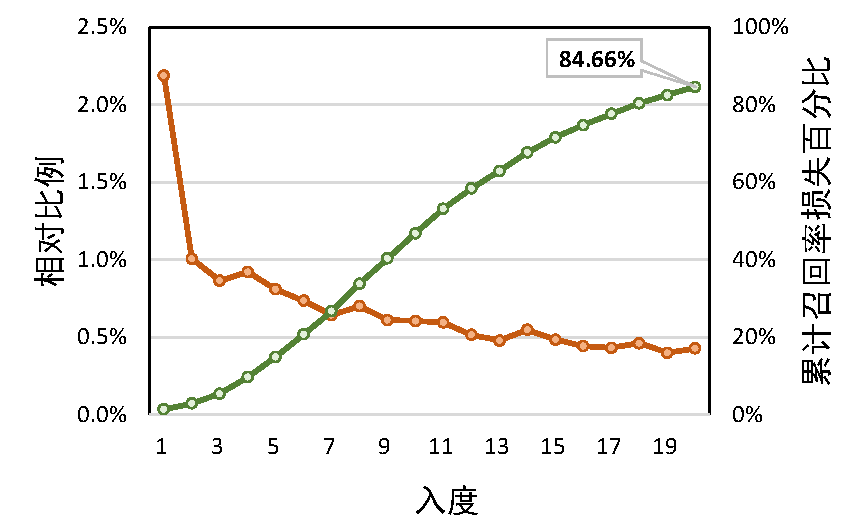
\includegraphics[width=0.7\textwidth]{figures/context-1/percent-in-degree.pdf}
  \caption{具有不同入度的点,对召回率损失的累积贡献曲线}
  \label{fig:percent-in-degree}
\end{figure}

本文指出,图连通性差的原因是由于现有构建算法的限制:即点的入度受其出度的限制。简单来说就是,为了保持图索引的高效性,一些点的出度会变小(通过近邻选择)。对于出度小的点,由于上述限制,它们的入度也小。接下来,本文将在\ref{sec:galg-connection}节中对这一限制的来源进行详细分析,并提出解决方案。


\subsection{搜索中存在冗余}
现有的最佳优先搜索算法在搜索过程中会产生较大的冗余,特别是在召回率较高的情况下。
正如本文在上一章节中所介绍的,$efs$参数是搜索算法中重要的超参数,它可以控制搜索速度和搜索精度(召回率)之间的权衡。总的来说,$efs$越大,精度越高,速度越慢。经过实验发现,$efs$参数与实际搜索过程中的迭代轮次(搜索步数)呈现出非常强的相关性。例如在$efs=200$的情况下,平均搜索步数为200.71,标准差为1.91。

因此为了简化问题的描述,本章节中的$efs$参数与搜索步数是相等的。为了便于叙述,本文首先定义\textit{最小搜索步数}:

\begin{definition}[最小搜索步数]
对于某个查询点$q_i$,在搜索步数$efs=s$下的召回率为$Recall_i$。那么存在一个保持$q_i$的召回率不降低的最小值$s$,那么$s$就是$q_i$在召回率为$Recall_i$的最小搜索步数。
\end{definition}
% 是搜索过程中结果队列的最大长度,每个查询的搜索步数数大致与$efs$成比例。

对于不同的查询点,其最小搜索步数差异很大。如图~\ref{fig:steps-histogram}所示,在DEEP1M数据集的查询集(有10000个查询点,详细见\ref{sec:galg-experiment}节)上,超过40\%查询点的最小搜索步数小于39。然而,现有的搜索算法对查询集中的所有查询点都设置相同的$efs$参数,在图~\ref{fig:steps-histogram}中这个值是300。
因此,现有搜索算法在搜索中就存在严重的冗余。对于上述那些最小搜索步数小于39的查询点,有87\%的搜索开销是冗余的(34.8\%的整体冗余开销)。接下来,我们将在\ref{sec:galg-earlystop}节中详细分析这个问题的原因,并提出我们的解决方案。

\begin{figure}[htbp]
  \centering
  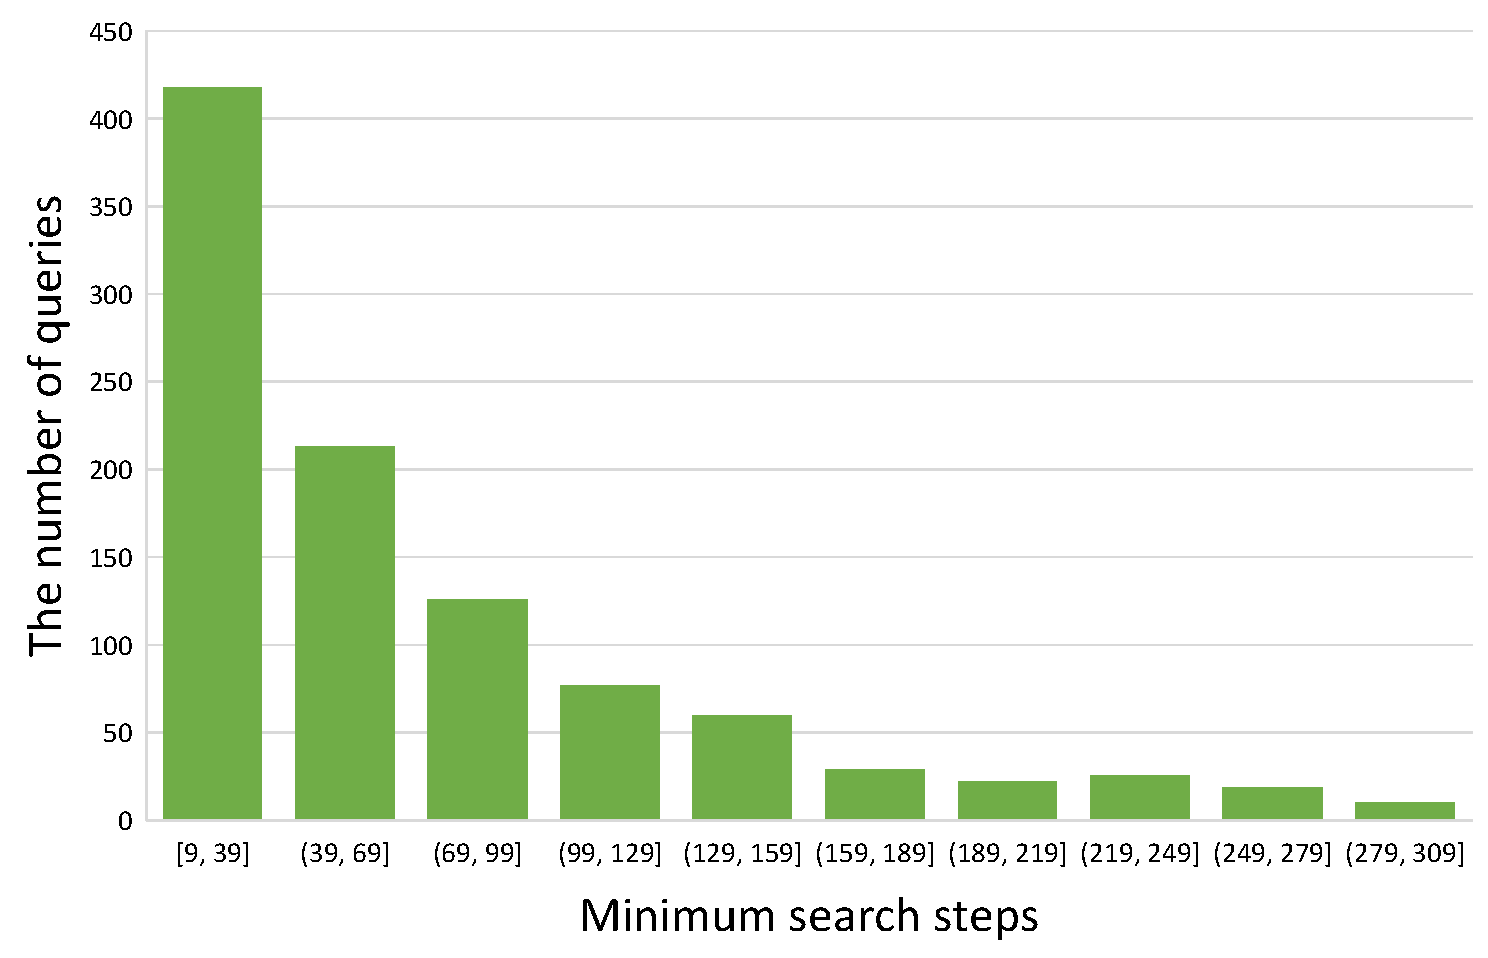
\includegraphics[width=0.7\textwidth]{figures/context-1/steps-histogram.pdf}
  \caption{查询集的最小搜索步数分布直方图\todo{重新画图}}
  \label{fig:steps-histogram}
\end{figure}

% todo:方法介绍?
\section{反向连接增强策略}\label{sec:galg-connection}
% TODO:表述到底是图还是图索引?
由于图中具有较小入度的点会对最终结果造成严重的精度影响,因此本节首先对整个HNSW图的入度和出度进行了分析,指出该问题的来源是现有构建算法不合理的限制。最后本文提出反向连接增强策略,有效减少这一问题导致的精度下降。

\subsection{度分析}
构建过程就是将数据集$X$中的数据点逐一添加到图上。如图~\ref{fig:idg-odg}所示,在时间$t_c$处,对应的待添加点是$x_c$(也称为插入点),此时对应的图是$G_c$。从点$x_c$的视角来看,整个构建过程可以分为两个部分:$t_c$之前和$t_c$之后。那么相应的,$x_c$的入度$IDG(x_c)$和出度$ODG(x_c)$也可以表示为两部分,如下公式所示:
\begin{equation}
  IDG(x_c) = IF1_{x_c} + IF2_{x_c}
\end{equation}
\begin{equation}
  ODG(x_c) = OF1_{x_c} + OF2_{x_c}
\end{equation}

\begin{itemize}
  \item $OF1_{x_c}$:在时间$t_c$之前$x_c$增加的出度。具体来说,当构建过程中插入点为$x_c$时(在图~\ref{fig:idg-odg}中$t_c$之前),在图索引$G_c$(在$t_c$之前)中找到$x_c$的$efc$最近点称为候选点。我们通过基于RNG的邻居选择策略选择其中的一部分作为$x_c$的邻居(即:$Neighbor(x_c)$),这些邻居的数量是$OF1_{x_c}$。
  \item $IF1_{x_c}$:在时间$t_c$之前$x_c$增加的入度。具体来说,在构建过程中插入点为$x_c$时(在图~\ref{fig:idg-odg}中为$t_c$之前),我们选择了$x_c$的当前邻居$Neighbor(x_c)$。对于$Neighbor(x_c)$中的每个点,当其邻居的数量小于$maxM0$时,我们还需要添加$x_c$作为其邻居。最终成功添加$x_c$作为邻居的点数是$IF1_{x_c}$,显然是$IF1_{x_c} \leq OF1_{x_c}$。
  \item $IF2_{x_c}$:在时间$t_c$之后$x_c$增加的入度。具体来说,当$x_c$已经在图中(在图~\ref{fig:idg-odg}中的$t_c$之后),$x_c$也可能成为其他插入点(绿色点)的候选点。如果点$x_c$最终成为了这些插入点的邻居,那么也就意味着$x_c$的入度会相应增加,增加的大小为$IF2_{x_c}$。
  \item $OF2_{x_c}$:在时间$t_c$之后$x_c$增加的出度。具体来说,当$x_c$已经在图索引中(在图~\ref{fig:idg-odg}中$t_c$之后),并且有一些点(黄色点)添加了$x_c$作为邻居。然后我们还需要将这些点添加为$x_c$的邻居,当$Neighbor(x_c)$的数量小于$maxM0$时。$x_c$的新邻居数量是$OF2_{x_c}$。
\end{itemize}

\begin{figure}[htbp]
  \centering
  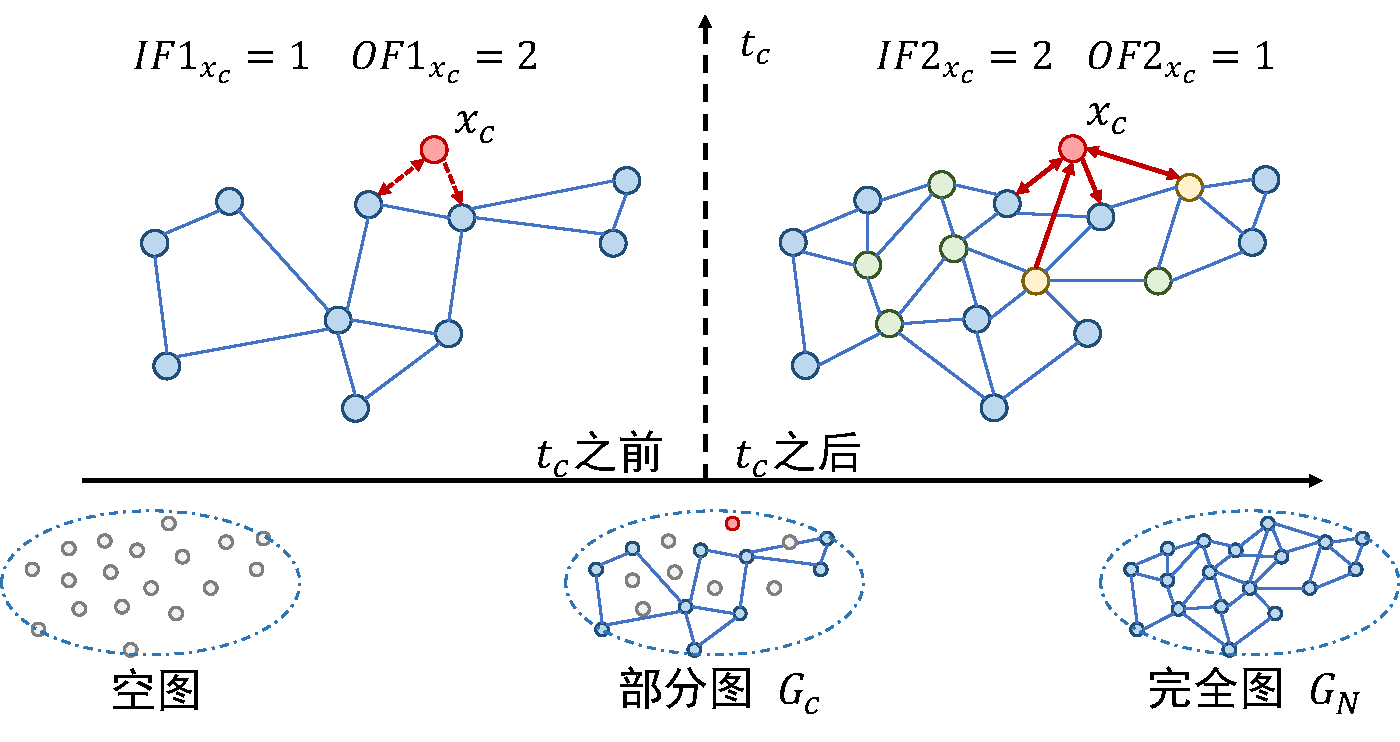
\includegraphics[width=0.7\textwidth]{figures/context-1/idg-odg.pdf}
  \caption{点$x_c$的入度和出度分别由两部分组成}
  \label{fig:idg-odg}
\end{figure}

\begin{figure}[tp]
  \centering
  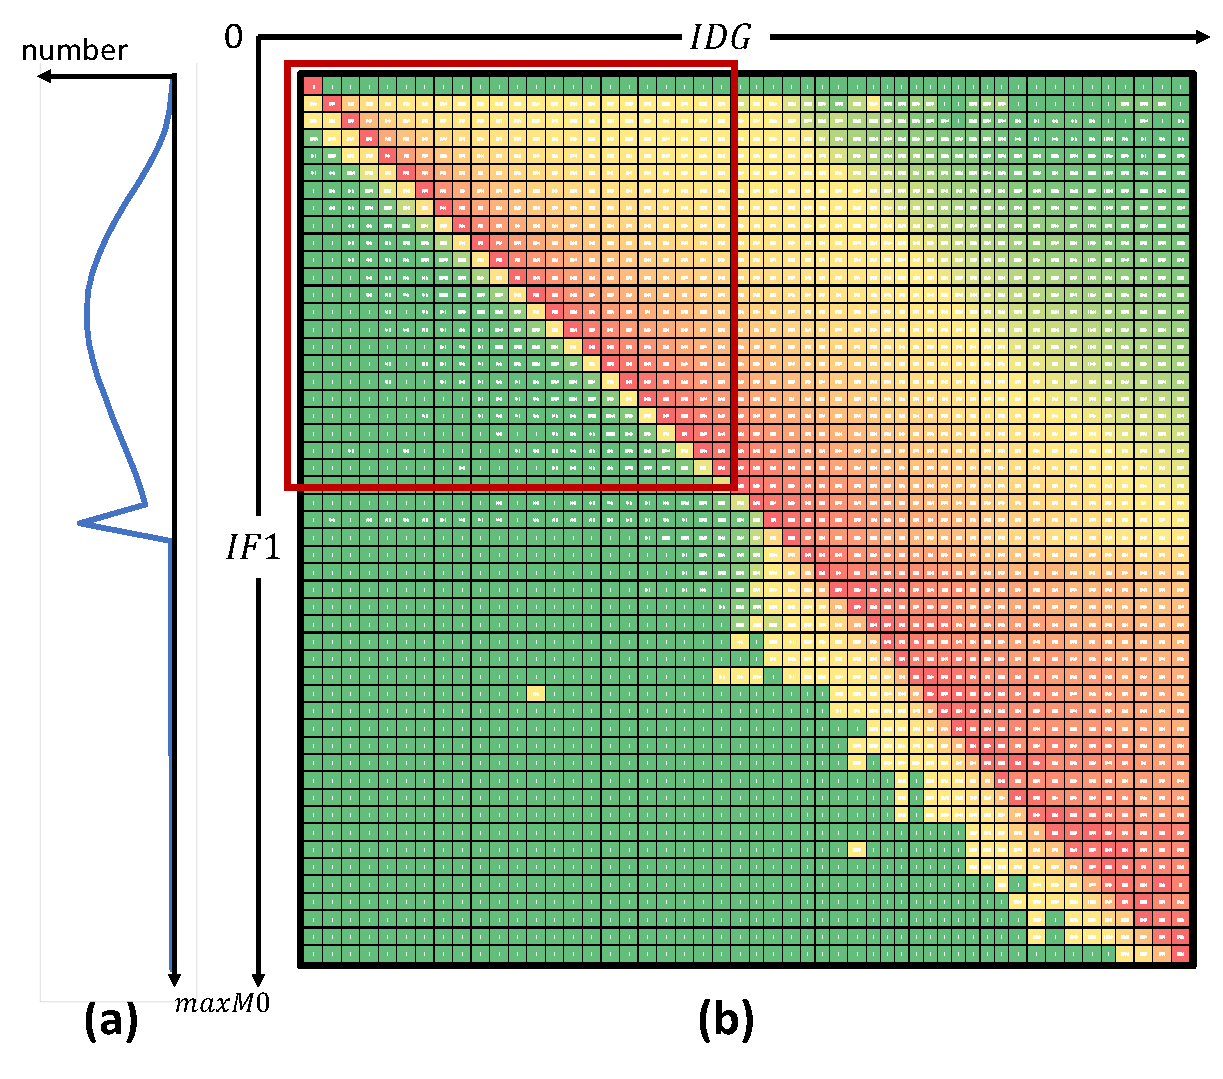
\includegraphics[width=0.6\textwidth]{figures/context-1/IF1-IDG.pdf}
  \caption{(a) $IF1$图索引上所有点的分布曲线(在Turing1M数据集上)。(b) $IDG$和$IF1$的热图,对于入度较小的点(在红框内),两者之间存在正相关关系。矩阵的每一行都按照(a)进行归一化。单个点的In-degree(约0.3 \textperthousand)非常大($\geq maxM0$),我们将它们截断。}
  \label{fig:if1-idg}
\end{figure}

如图~\ref{fig:idg-odg}所示, $IF2_{x_c}$和$OF2_{x_c}$取决于$x_c$是否可以被其他点(绿色点)找到。显然,入度$IF1_{x_c}$在$t_c$上的值越大,在$t_c$之后发现$x_c$的概率就越大。图~\ref{fig:if1-idg}(b)展示了$IDG$和$IF1$之间的关系。如果某些点(红框内)的$IF1$很小,那么它们最终入度$IDG$也很小。也就是说,$IDG$和$IF1$之间存在正相关关系。

在完整图$G_N$中的点$x_c$的连通性很大程度上取决于$IF1_{x_c}$。同时,$IF1_{x_c}$与$OF1_{x_c}$之间存在着一种\textbf{制约关系},即$IF1_{x_c} \leq OF1_{x_c}$。基于RNG的近邻选择策略尽管可以保持图上搜索\cite{hnsw-2018}的较高效率,但是忽略了对于这些入度较小点的关注。这导致了80.5\%的点$OF1$小于$maxM0$的2/5(如图~\ref{fig:if1-idg}(a),因为$IF1$和$OF1$的分布几乎相同)。也就是说,$IF1_{x_c}$与$OF1_{x_c}$之间存在制约关系,最终导致图$G_N$的连通性差。

\begin{algorithm}[tp]
  \caption{反向连接增强算法}
  \label{alg:enhancement} 
  \begin{algorithmic}[1]
      \REQUIRE
      底库数据集 $X$, 最大邻居数 $maxM0$, 起始点 $p_s$
      \ENSURE
      图索引 $G_N$
      \FOR{ $p_{in} \in X$}
      \STATE $Q_{cand}^{in} \gets$ greedy search$(q,G_s,p_s,efc,efc)$
      \STATE $Q_{sel}^{in} \gets$ SelectNeighborByRNG$(p_{in},Q_{cand}^{in},maxM0)$
      \STATE $setNeighbor(p_{in}) \gets Q_{sel}^{in}$
      \STATE $Q_{add} \gets Q_{cand}^{in} \setminus Q_{sel}^{in}$
      \FOR{ $p_r \in Neighbor(p_{in})$}
      \STATE $addNeighbor(pr) \gets p_{in}$
      \ENDFOR
      
      \WHILE{$Indegree(p_{in}) < maxM0$}
      \STATE $p_r \gets Q_{add}$
      \STATE $addNeighbor(pr) \gets p_{in}$
      \ENDWHILE
      \ENDFOR
      \RETURN $G_N$
  \end{algorithmic} 
\end{algorithm}

\subsection{我们的方法}
为了解决上述问题,本文提出了反向连接增强策略。我们对入度小的点增加了一些连接,使$IF1$打破了与$OF1$的限制关系。简单来说,点$x_c$的入边不仅从其邻居中选择,而且从其候选点中也考虑一部分,由于候选点是已经计算过的,因此也不会导致额外的计算开销。这一策略的伪代码如算法~\ref{alg:enhancement}所示。

图~\ref{fig:enhence}直观地展示了反向连接增强策略,$x_c$是构建过程中的插入点,($x_1$, $x_2$, $x_3$)是$x_c$的候选集。然后通过基于RNG的邻居选择策略选择$x_1$和$x_3$作为$x_c$的邻居。我们的方法和之前的方法的区别主要体现在$IF1_{x_c}$。因为$x_2$和$x_4$比$x_c$更接近$x_3$,所以$x_c$不属于$Neighbor(x_3)$。由于$OF1_{x_c}$受限于$IF1_{x_c}$,以前的方法只能通过$x_1$找到$x_c$,这意味着其他点很难找到$x_c$。
我们的方法打破了$IF1_{x_c}$和$OF1_{x_c}$之间的限制关系,从$x_c$的候选点中选择一些点(如$x_2$),然后将$x_c$作为$x_2$的邻居(用紫色的边连接)。然后我们可以通过$x_1$或$x_2$点找到$x_c$。与之前的方法相比,该方法极大地提高了图的连通性。详细的比较结果显示在\ref{sec:galg-experiment}部分。

\begin{figure}[htbp]
  \centering
  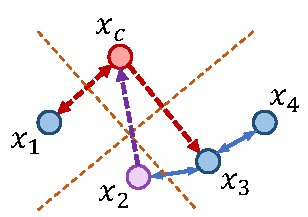
\includegraphics[width=0.4\textwidth]{figures/context-1/enhance.pdf}
  \caption{反向连接增强策略。之前:只能通过点$x_1$找到点$x_c$,现在:通过点$x_1$或点$x_2$都可以找到点$x_c$。}
  \label{fig:enhence}
\end{figure}


\section{查询感知早停策略}\label{sec:galg-earlystop}
现有的最佳优先搜索算法在搜索过程中会产生较大的冗余,特别是在召回率较高的情况下。其原因是不同的查询点所处的图区域不同,因此对于不同的查询都采用相同的搜索步数会造成严重的计算冗余问题。本节首先对这一问题进行分析,指出查询之间的最小搜索步数的差异来源是由于所处图区域的连接特点不同。然后提出查询感知早停策略,可有效减少搜索算法在召回率较高情况下的冗余。

\subsection{分析}
本文指出,查询在图上的区域连接关系导致了冗余搜索问题,区域是指图中靠近查询的部分。对于相同的查询,其最小搜索步数在不同的图上的差异很大。
图~\ref{fig:min-step}显示了查询向量的最小搜索步数的分布(在DEEP1M数据集上),水平轴和垂直轴分别对应两个不同的图索引。这两个图索引具有相同的基向量和参数,并且在构建过程中只改变插入点的顺序。我们发现对于相同的查询,其最小搜索步数之间有巨大的差异(例如,3到190)。
\begin{figure}[htbp]
  \centering
  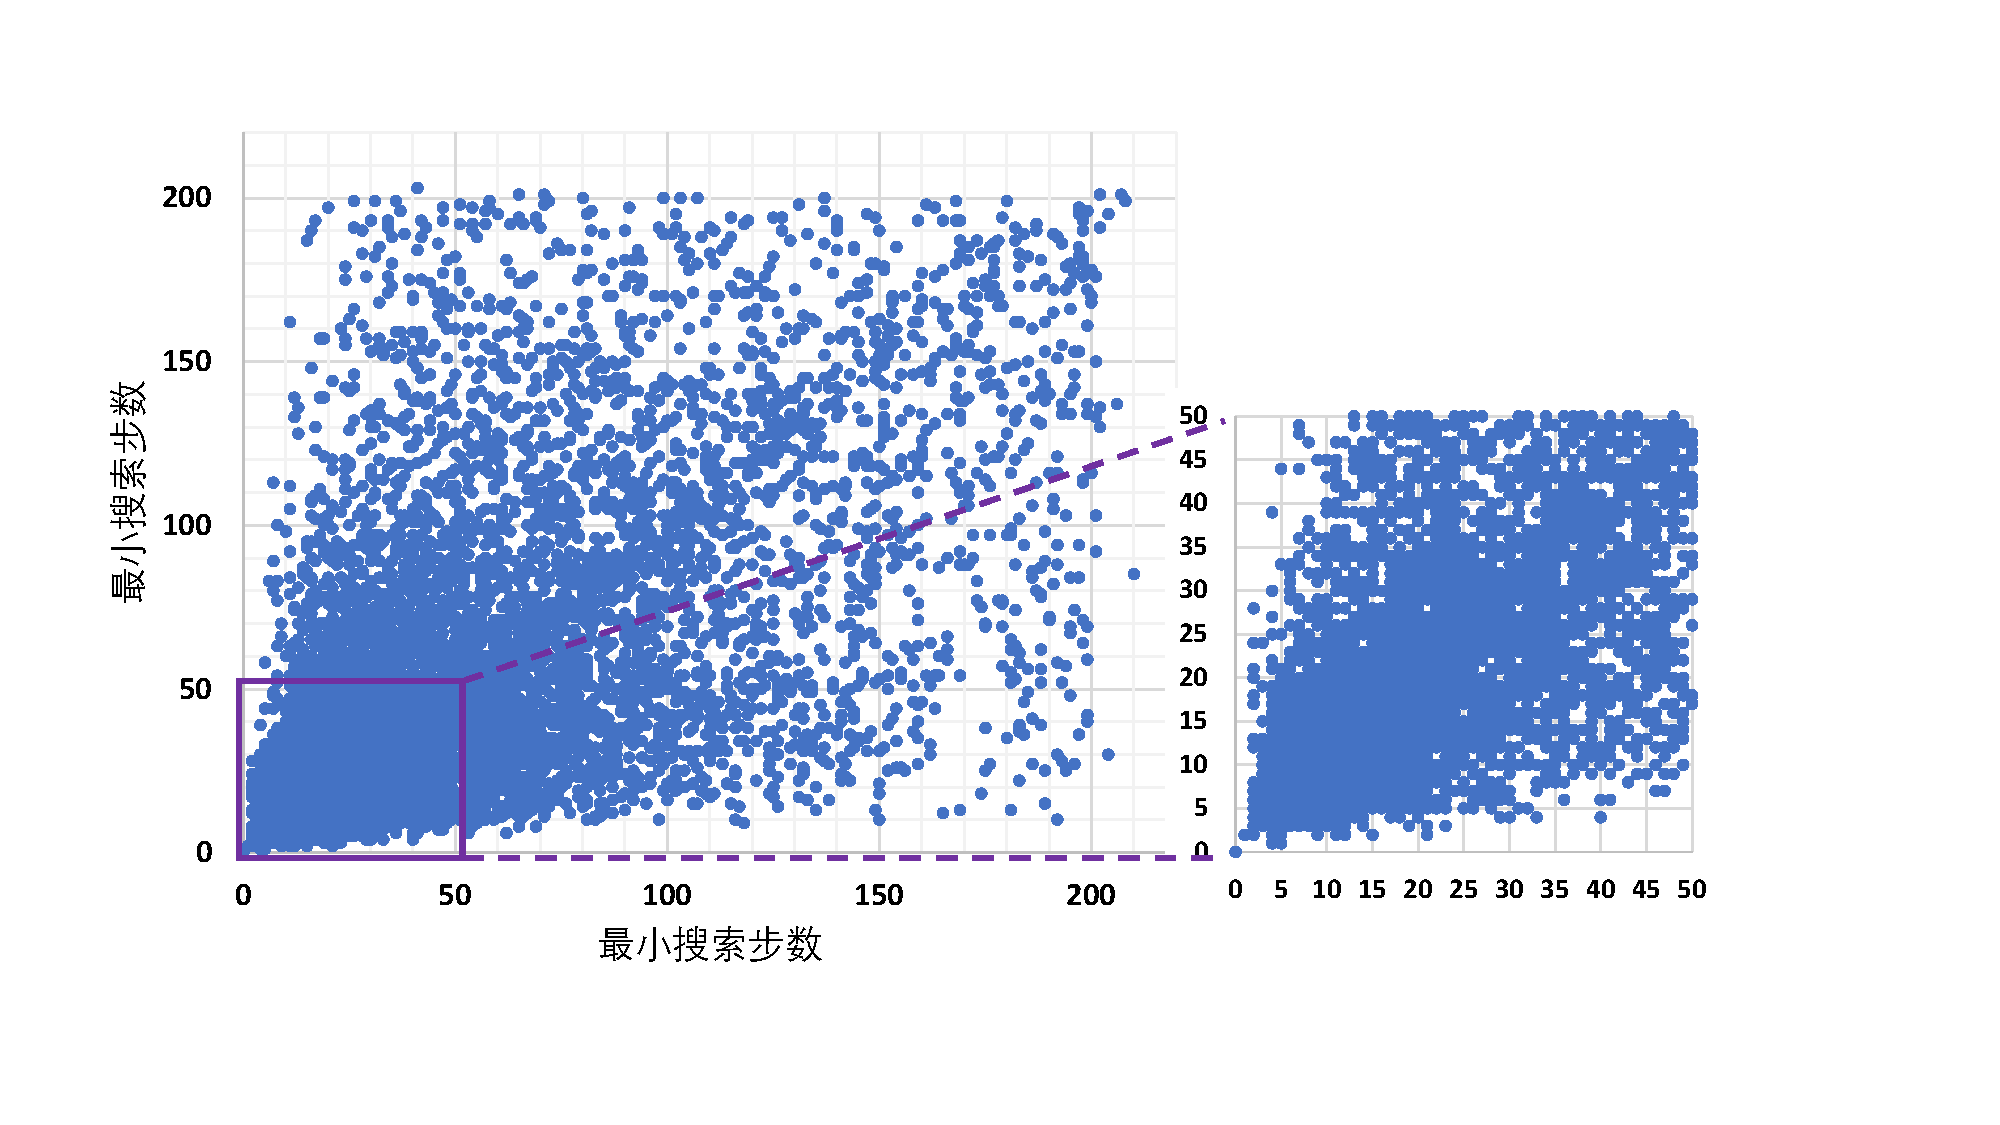
\includegraphics[width=0.9\textwidth]{figures/context-1/min search step.pdf}
  \caption{查询向量的最小搜索步数分布在两个不同的图索引中}
  \label{fig:min-step}
\end{figure}

根据连接关系的特点,区域可分为两种类型:对称连接区域(图~\ref{fig:grid}(a))和非对称连接区域(图~\ref{fig:grid}(b))。对称连接是指某一点的邻居在空间中均匀分布。非对称连接是指某一点的邻居在空间上不均匀分布。
与对称连接区域相比,非对称连接区域需要更多的搜索步数才能达到相同的召回率。 
当当前搜索点非常接近查询时。对于对称连接区域,当前搜索点可以快速地对查询的附近区域进行完整的探索。因此,对称连接区域可以以较少的搜索步数找到查询的所有最近点。对于非对称连接区域,由于查询附近的点之间缺乏连接,当前搜索点会采取一些“绕路”的方式来寻找所有与查询最近的点。 如图~\ref{fig:grid}所示,$q_a$的最小搜索步数仅为7步,$q_b$的最小搜索步数高达17步。如果我们想要得到同样高的召回率,那么在$q_a$的搜索开销中存在冗余。
\begin{figure}[tp]
  \centering
  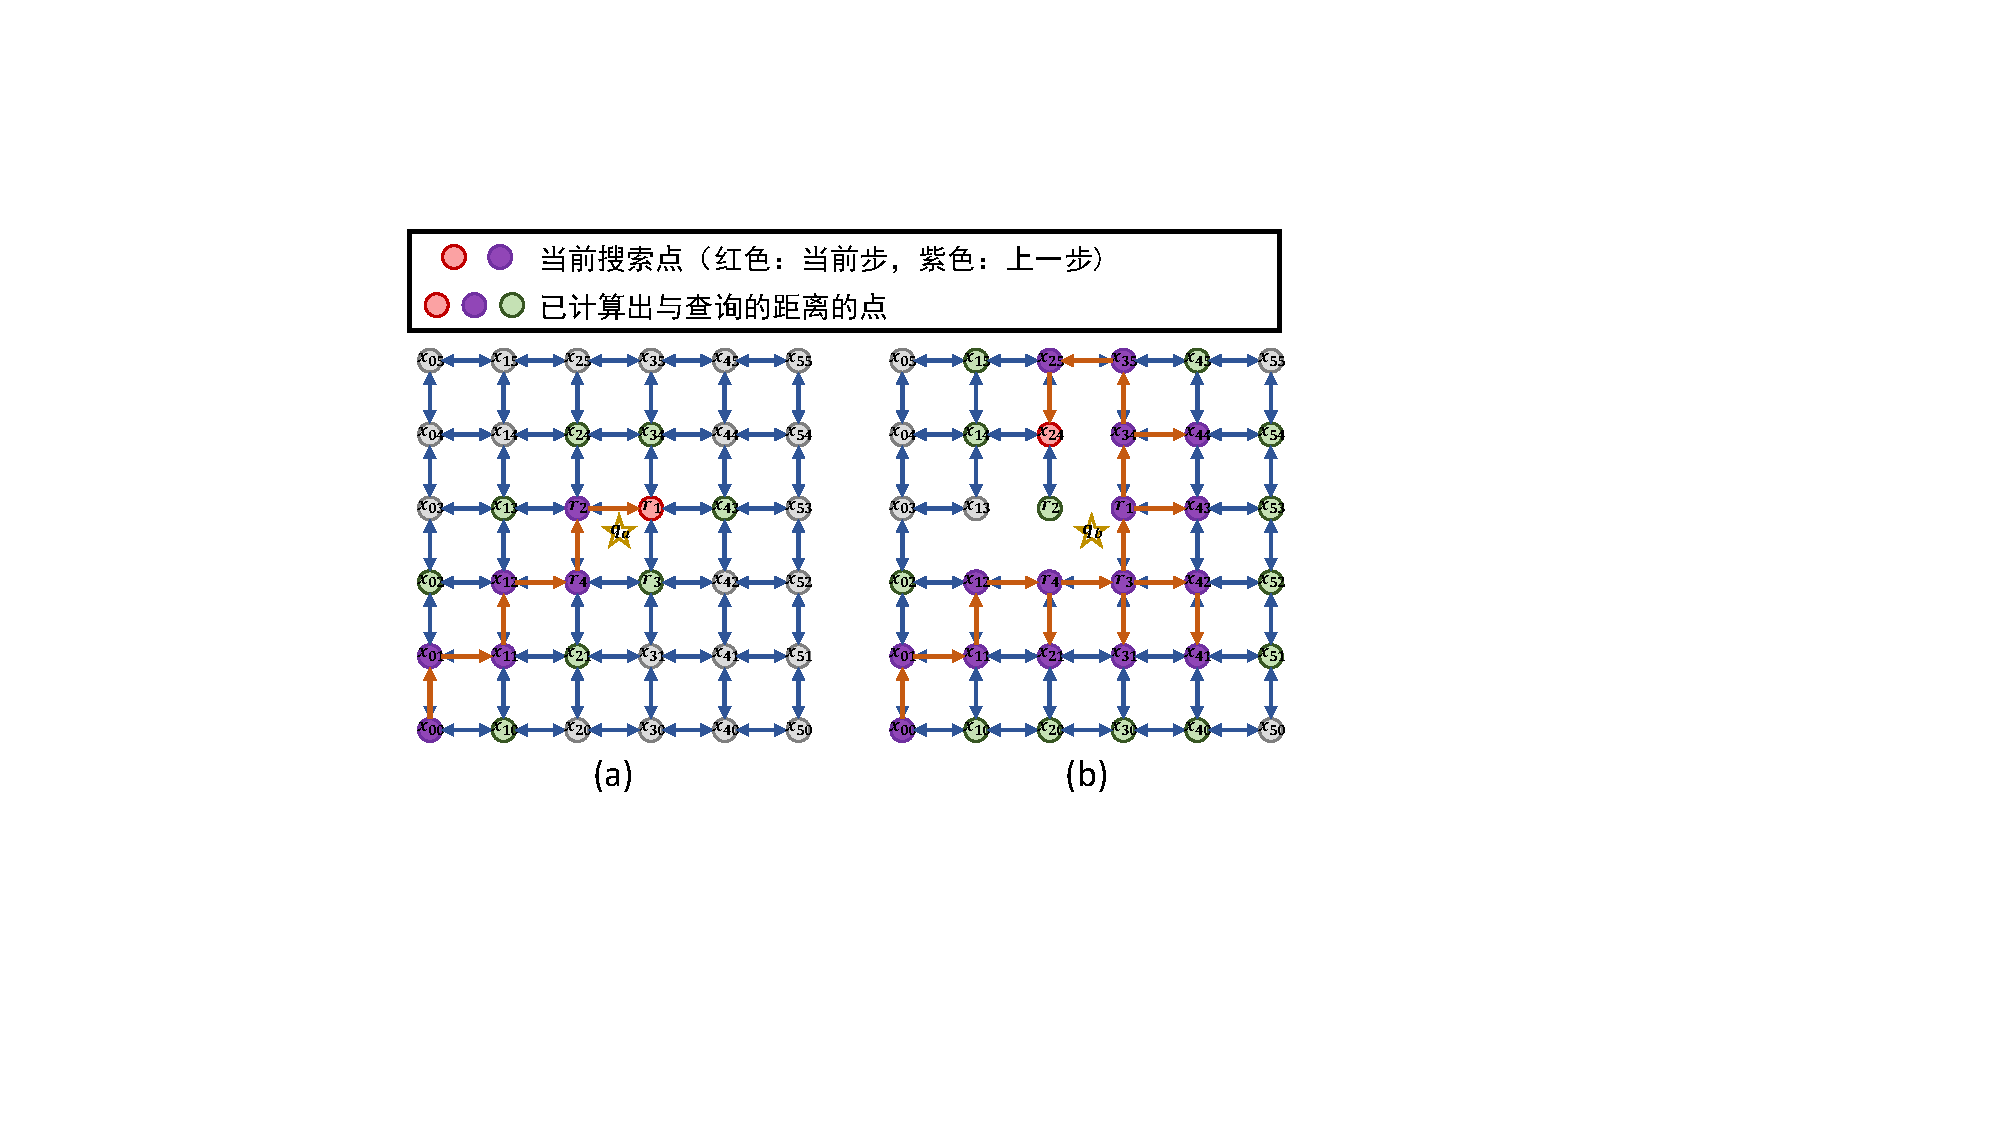
\includegraphics[width=0.6\textwidth]{figures/context-1/grid.pdf}
  \caption{在图索引上搜索查询最近邻的示意图。(a)当查询$q_a$位于一个对称连接区域时,可以很容易地找到它的所有最近邻居。(b)当查询$q_b$位于非对称连接区域时,我们需要更多的搜索步数来找到所有的最近邻居。}
  \label{fig:grid}
\end{figure}

由于高维空间中的连接关系非常复杂,从构建算法上很难解决该问题。因此,本文从搜索算法的角度来解决这个问题。
我们定义两个变量$d_{pop}$和$d_{topk}$来识别区域的连接关系。这里的距离是指某个点与查询之间的距离。对于搜索过程的每个步骤,$d_{pop}$表示当前搜索点的距离,$d_{topk}$表示从结果队列中$k$ -th最近的点到查询的距离。

我们通过在搜索过程中$d_{pop}$和$d_{topk}$的变化来识别这两种类型的区域。当当前搜索点非常接近查询时,如果曲线$d_{pop}$相对于曲线$d_{topk}$是光滑的,则意味着区域连接关系是对称的。
对于对称连接区域,由于邻居分布非常均匀,靠近查询的点将被添加到搜索队列中。因此,曲线$d_{pop}$相对于曲线$d_{topk}$是光滑的(如图~\ref{fig:search-path}(a)所示)。
对于非对称连接区域,由于点的近邻分布不均匀,导致该区域内部分点之间没有连接。在这种情况下,在接下来的每个步骤中,$d_{pop}$首先递增。然后HNSW会找到一个离当前搜索点更近的点通过“绕路”,$d_{pop}$会下降。因此在曲线$d_{pop}$(如图~\ref{fig:search-path}(b)所示)上会有一些波动。

我们用图~\ref{fig:grid}进一步说明这一点。对于查询$q_a$,当使用点$r_1$作为当前搜索点时,由于连接的区域$a$是对称的,搜索过程会以$q_a$为中心向外扩散。当前搜索点与查询$q_a$在区域a上的距离变化类似于图~\ref{fig:search-path}(a)中的曲线$d_{pop}$。
对于查询$q_b$,当使用点$r_1$作为当前搜索点时,由于$b$区域的连接是非对称的(点$r_2$不在搜索队列中),搜索过程相对于$q_b$会在右下和右上方向扩散。我们无法找到$r_2$直到点$x_{24}$和查询$q_b$之间的距离计算出来。当前搜索点与查询$q_b$在区域b上的距离变化类似于图~\ref{fig:search-path}(b)中的曲线$d_{pop}$。

\begin{figure}[tp]
  \centering
  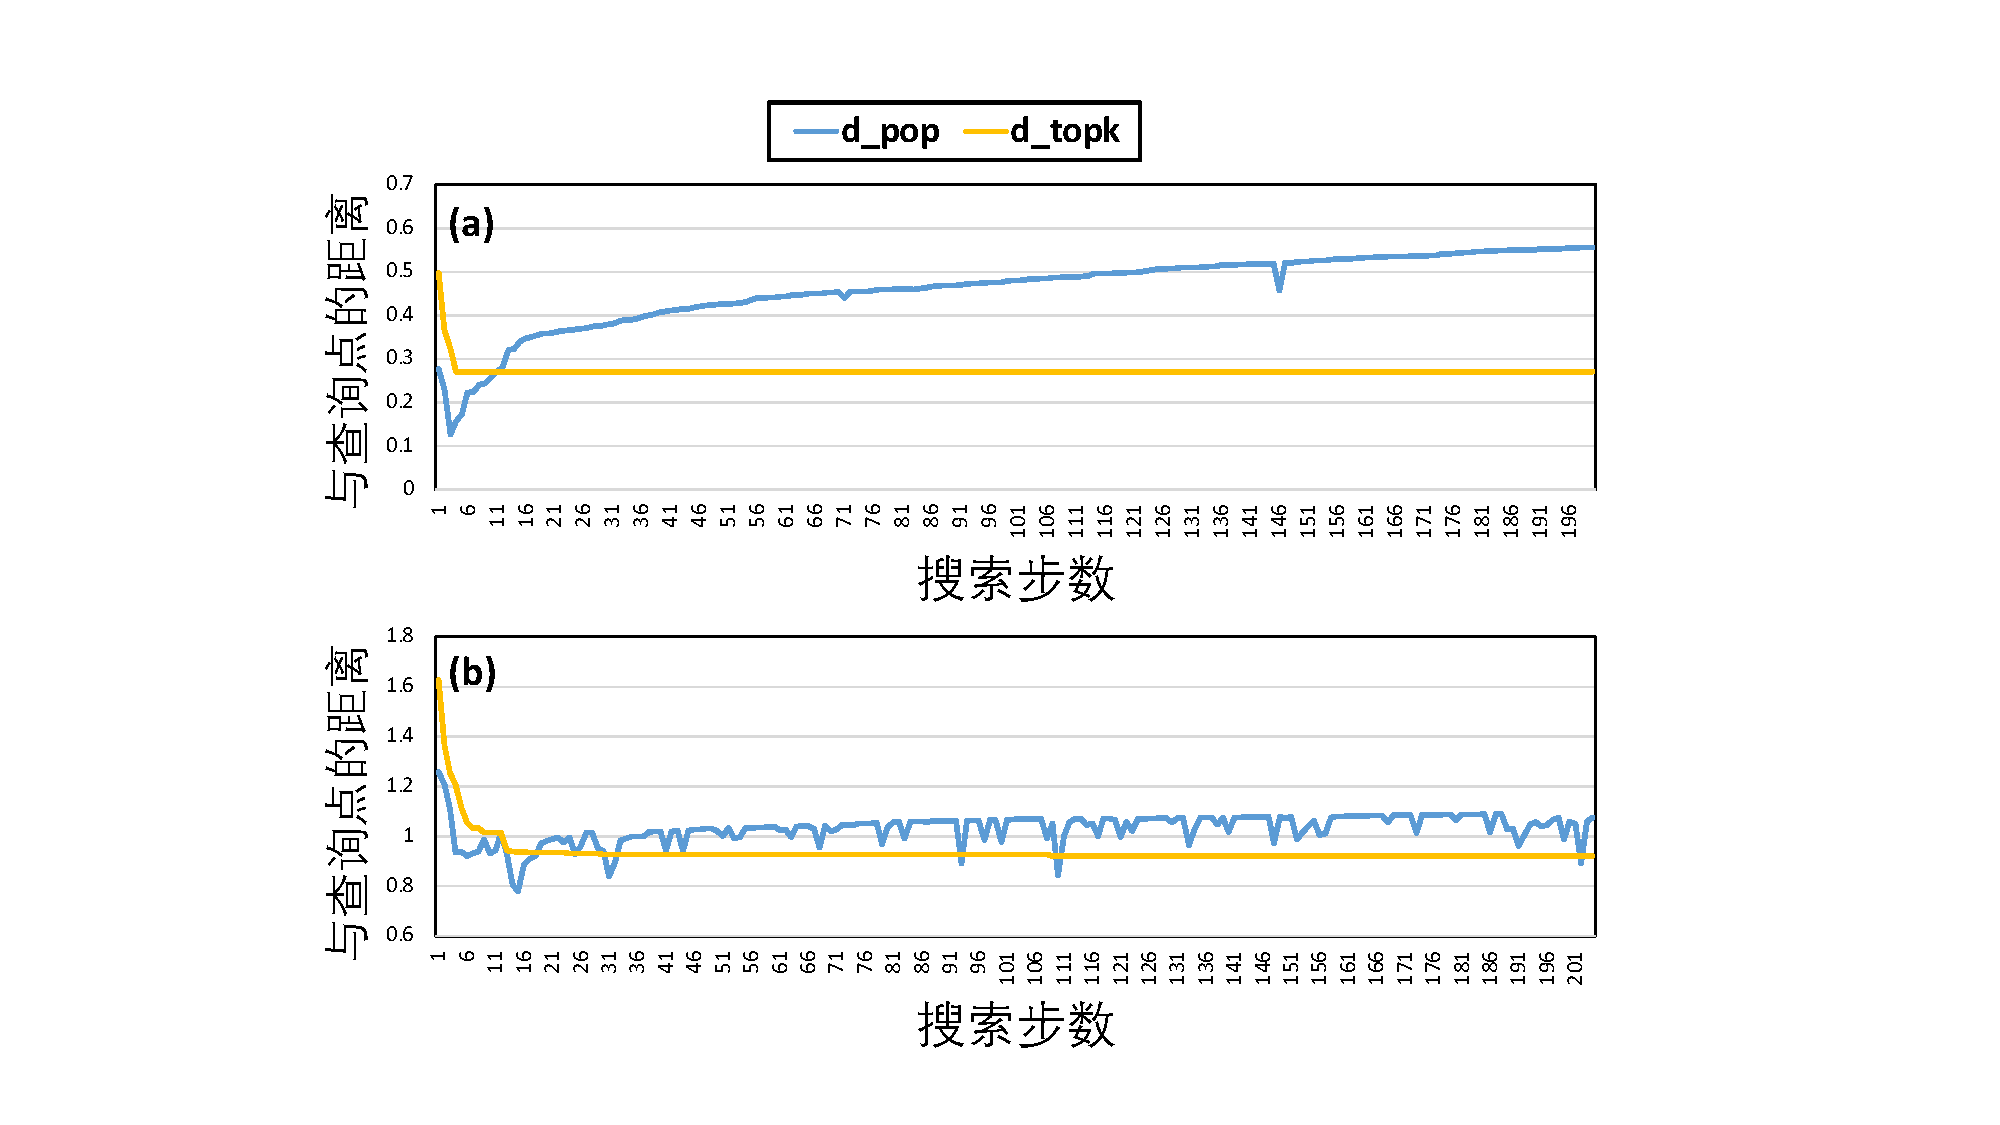
\includegraphics[width=0.6\textwidth]{figures/context-1/dist-feature.pdf}
  \caption{在搜索过程中(在DEEP1M数据集上)两个代表性查询的$d_{pop}$和$d_{topk}$的变化。(a)查询位于对称连接区域,其最小搜索步长为6。(b)查询位于非对称连接区域,其最小搜索步数为200步。}
  \label{fig:search-path}
\end{figure}

\subsection{我们的方法}
为了解决搜索过程中的冗余问题,提出了查询感知早停策略。在上述分析的基础上,我们指出$d_{pop}$相对于$d_{topk}$的曲线特征可以用来在搜索过程中识别区域。

我们通过分析$d_{pop}$相对于$d_{topk}$在搜索过程中的曲线平滑性,设计了一个预测模型来决定是否提前停止。为了消除每个查询与其最近邻居之间不一致的影响,我们另外考虑$d_{top1}$特征。我们使用的特征如下:
\begin{itemize}
    \item $d_{pop}$:当前步中,当前搜索点与查询点之间的距离。
    \item $d_{topk}$:当前步结束后,结果队列中离查询最近的点$k$ -th的距离。
    \item $d_{top1}$:当前步结束后,结果队列中最近的点到查询的距离。
\end{itemize}

对于完整的工作流(如图. \ref{fig:aware-workflow}所示),我们不需要向图索引添加任何额外的结构。在训练阶段(图~\ref{fig:aware-workflow}(a)),我们使用学习向量作为训练集(也将其划分为验证集)。对于训练集中的每个数据,我们都将按照上述搜索算法执行一个完整的搜索过程。
我们可以很容易地得到每一步的距离($d_{pop}$, $d_{topk}$和$d_{top1}$),作为预测模型的训练特征。然后我们计算最小搜索步长,并将其与曲线长度进行比较以获得标签。Label =1表示“继续搜索”,Label =0表示“终止搜索”。
在推理阶段(图~\ref{fig:aware-workflow}(b)),我们收集搜索过程中的动态特征,并通过训练好的预测模型预测剩余的搜索步数。
\begin{figure}[tp]
  \centering
  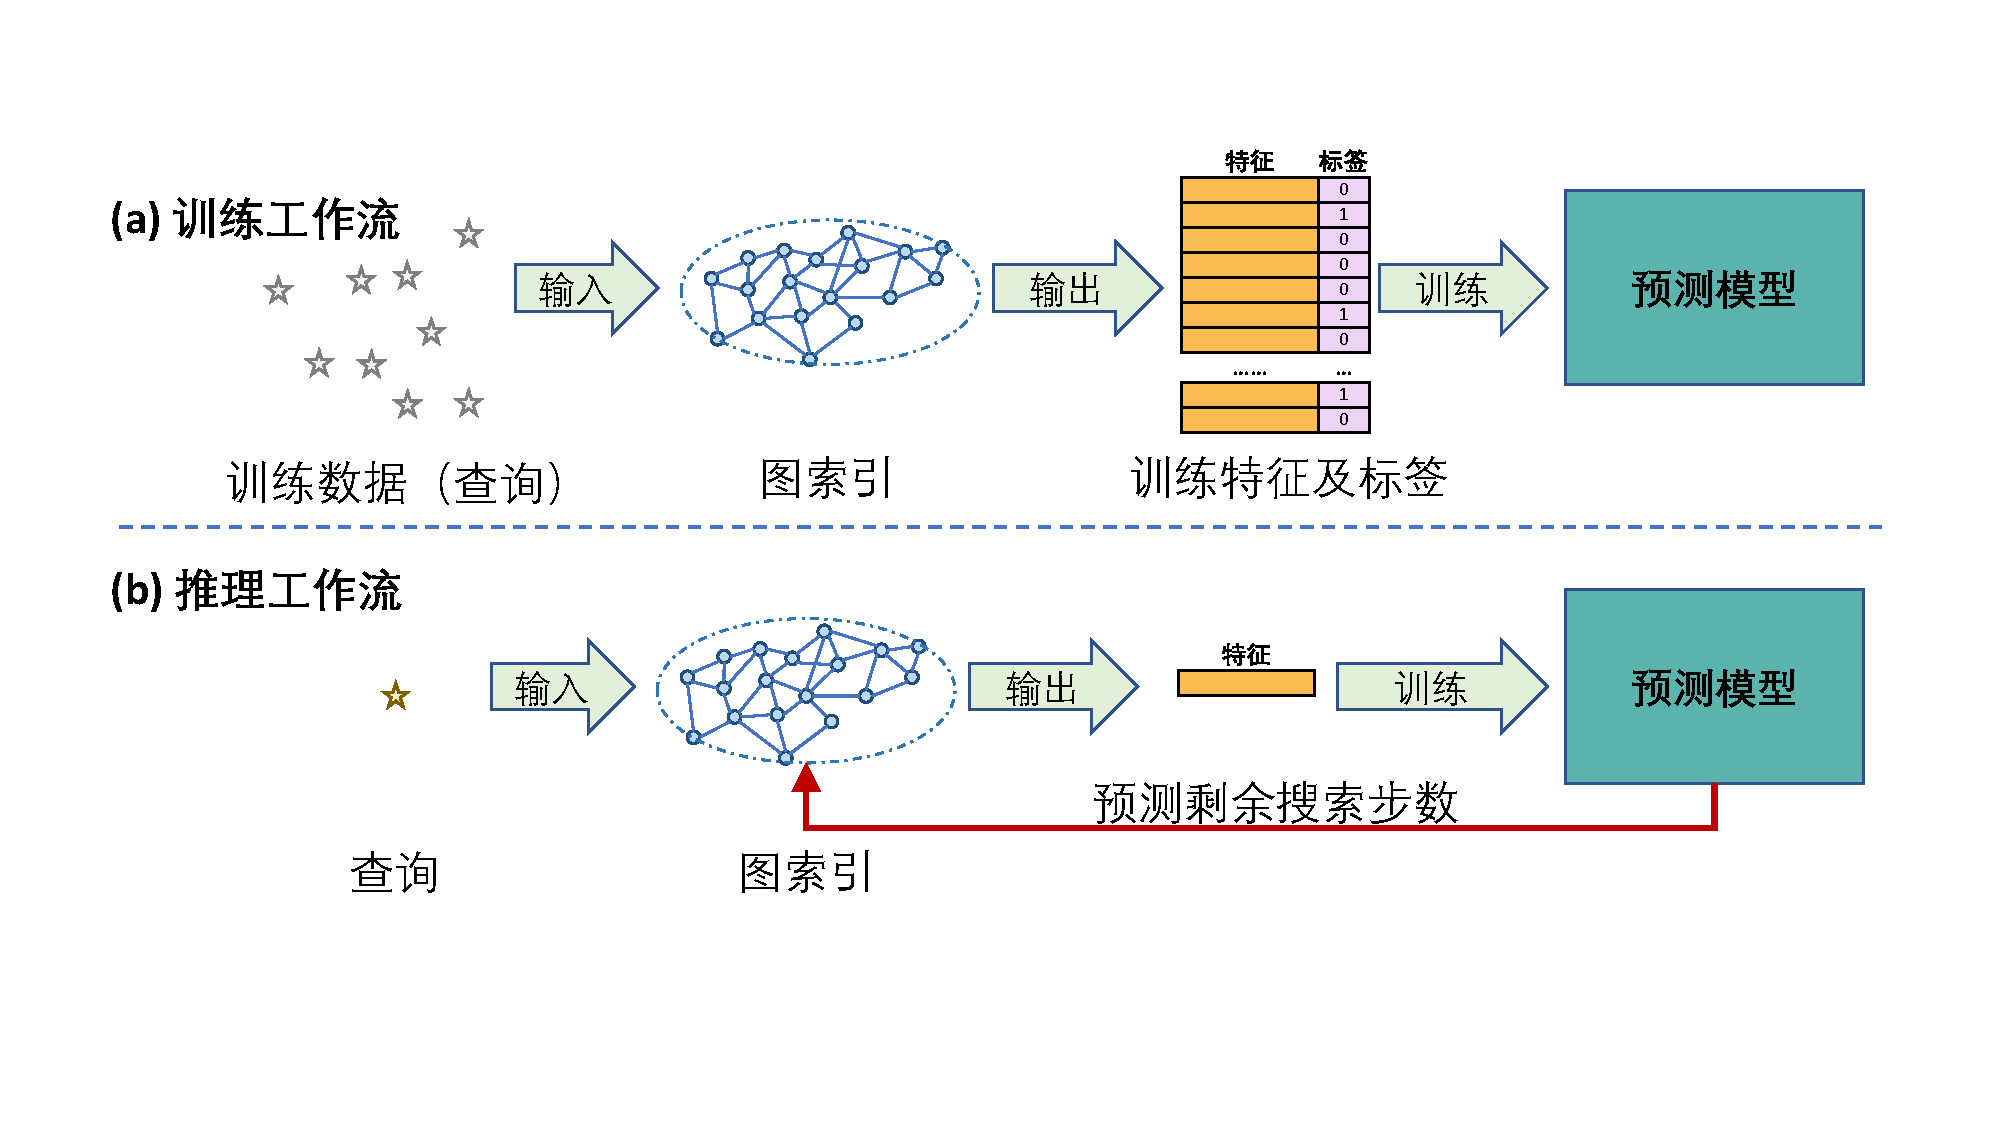
\includegraphics[width=0.7\textwidth]{figures/context-1/aware-workflow.pdf}
  \caption{支持查询感知的早停策略的工作流。(a)训练工作流,首先使用采样数据在图索引上进行搜索,然后在搜索过程中使用得到的动态特征来训练预测模型。(b)推理工作流,将训练好的模型集成到图索引框架中,在查询搜索过程中动态预测剩余搜索步数。}
  \label{fig:aware-workflow}
\end{figure}

预测模型的训练过程主要通过分析$d_{pop}$序列的平滑性来决定是否停止搜索过程。具体过程如下:(1)求$d_{pop}$曲线与$d_{topk}$曲线的上升交点步长。如果从$st_{stable}$ -th阶跃开始,$d_{pop}$大于$d_{topk}$,则$st_{stable}$称为上升交叉阶跃。(2)获取$d_{pop}$序列。从$st_{stable}$ -th步骤开始,在接下来的每一步中,$d_{pop}$添加到$d_{pop}$序列中,直到$d_{pop}$和$d_{topk}$之间的差大于$d_{topk}$和$d_{top1}$之间的差。(3)对$d_{pop}$序列进行逐差运算。对于$d_{pop}$序列,我们对其进行$n$逐差运算(类似于连续曲线的$n$阶导数)。(4) $d_{pop}$序列的方差与阈值比较。最后,我们计算$d_{pop}$序列的方差,并将其与一定阈值$th_{dist}$进行比较。如果大于阈值,则输出“继续搜索”,否则输出“终止搜索”。在实际搜索过程(推理阶段)中,我们可以轻松地收集这些距离作为预测的特征。

\begin{figure}[tp]
  \centering
  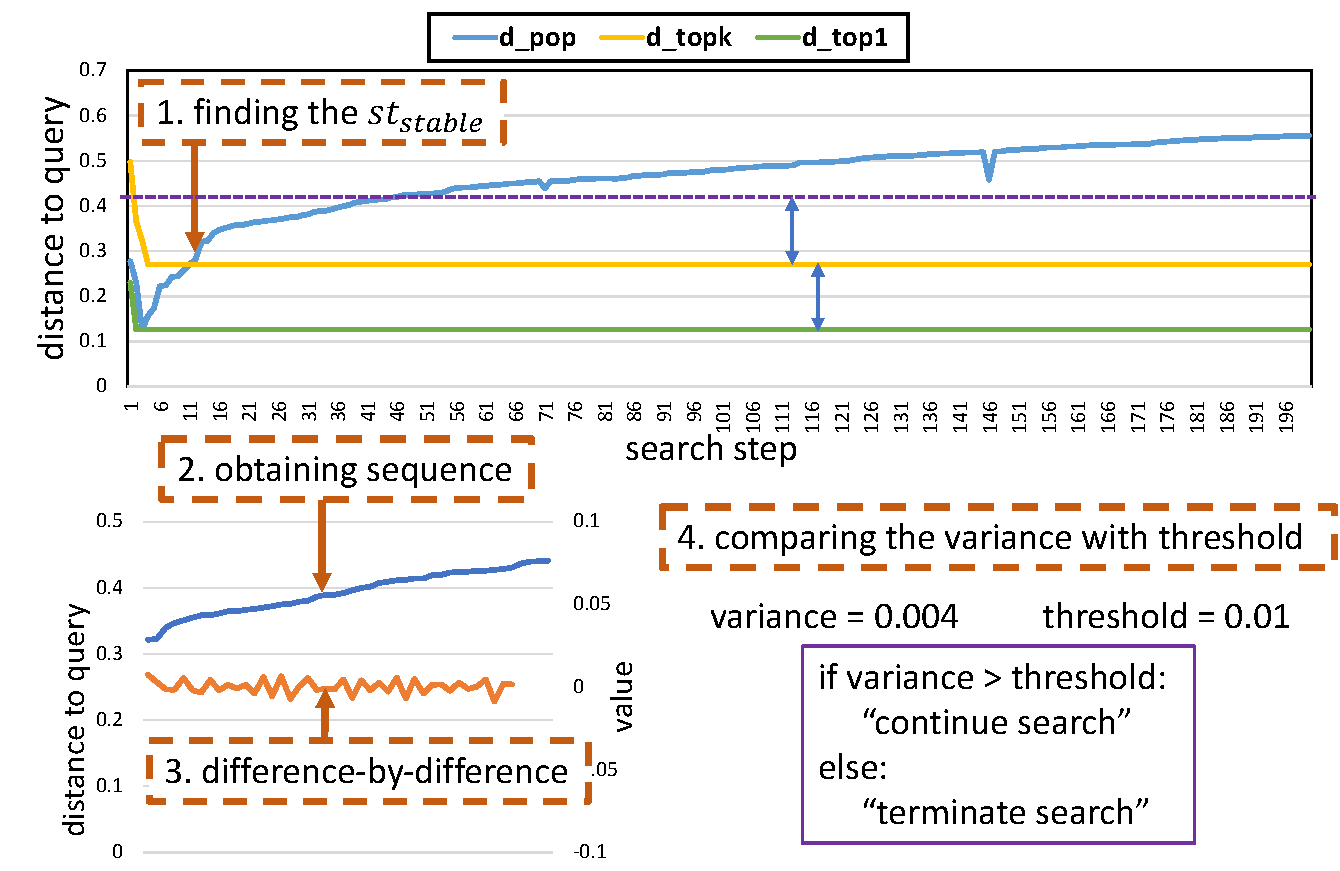
\includegraphics[width=0.7\textwidth]{figures/context-1/prediction model.pdf}
  \caption{预测模型的整个流程。它由4个步骤组成:(1)找到$st_{stable}$,(2)获得序列,(3)逐差,(4)方差与阈值比较。}
  \label{fig:prediction-model}
\end{figure}


\section{实验结果}\label{sec:galg-experiment}
在本节中,我们首先将我们的方法与最先进的近似近邻搜索方法进行比较。通过消融研究进一步分析每种技术的贡献。对于每个数据集和方法,进行多次实验,以获得稳定可靠的结果。

\subsection{实验设置和数据集}
\subsubsection{数据集}
我们使用的数据集如表~\ref{tab:datasets}所示,这些数据集在近似近邻搜索方法中被广泛使用。\ganns 方法将基础数据构建为图索引,并在该图索引上搜索查询数据的$k$最近邻。原始数据集包含10亿数据,我们截取前100万/ 1000万数据作为底库数据集。对于DEEP数据集,我们从其余数据中截取一些数据作为训练数据集(用于训练预测模型)。
\begin{itemize}
    % \item SIFT1M/10M \footnote{\label{bigann}http://corpus-texmex.irisa.fr/}: SIFT dataset consists of SIFT descriptors extracted from a large image dataset, and each data is a 128-dimensional vector.
    \item DEEP1M/10M \cite{deep-2016}:DEEP数据集来自深度分类图像模型GoogLeNet,每个数据都是一个96维向量。
    \item Turing1M/10M \cite{billionanns}:Turing数据集是由微软图灵团队为十亿规模的近似近邻搜索挑战赛发布的新数据集。它由图灵AGI v5编码的Bing查询组成,每个数据都是一个100维向量。
    % \item GIST1M \footref{bigann}: GIST dataset consists of GIST descriptors extracted from a image dataset, and each data is a 960-dimensional vector.
\end{itemize}

\begin{table}[htbp]
  \centering
  \caption{数据集信息}
  \label{tab:datasets}
  \begin{tabular}{ccccc}
  \hline
  数据集名称      & 数据维度   & 底库数据集大小   & 训练集大小 & 查询集大小 \\ \hline
  % SIFT1M/10M   & 128 & \begin{tabular}[c]{@{}c@{}}1,000,000/\\ 10,000,000\end{tabular} & -     & 10,000     \\
  DEEP1M/10M   & 96  & \begin{tabular}[c]{@{}c@{}}1,000,000/\\ 10,000,000\end{tabular} & 100,000     & 10,000     \\
  Turing1M/10M & 100 & \begin{tabular}[c]{@{}c@{}}1,000,000/\\ 10,000,000\end{tabular} & -   & 100,000    \\ \hline
  % GIST1M       & 960 & 1,000,000                                                       & -           & 1,000      \\ \hline
  \end{tabular}
\end{table}

\subsubsection{基线算法}
对于的基线方法,我们在Github上采用了他们的代码,并按照他们的建议设置相关参数。在搜索过程中,我们都使用一个线程来比较算法。在构建过程中,为了节省时间,我们使用所有线程构建所有索引。
\begin{itemize}
    \item \textbf{HNSW}\footnote{https://github.com/nmslib/hnswlib}是一种著名的基于图的算法,它基于一种称为分层NSW图的结构。
% \item \textbf{DPG}\footnote{https://github.com/DBAIWangGroup/nns\_benchmark} is based on a $k$NN graph to reselect undirected edges.
    \item \textbf{NSG}\footnote{https://github.com/ZJULearning/nsg}基于$k$ NN图,然后以导航节点为起点构建展开图。
\end{itemize}

\subsection{整体性能}
在多个数据集上对最先进的算法(HNSW和NSG)和本文所提出方法进行了实验。对于NSG,我们根据其在Github上的建议设置DEEP和Turing数据集的参数(由于它们的维度相似)。在实验中,对所有数据集设置如下参数:$L$ = 40, $R$ = 50, $C$ = 500。对于HNSW,通过网格搜索为每个数据集选择搜索性能最好的参数。在实验中,对所有数据集设置如下参数:$M$ = 20, $maxM0$ = 40, $efc$ = 300。

图~\ref{fig:exper-total}显示了我们的方法与当前最先进算法的整体性能对比结果。我们分别在四个数据集(DEEP1M, DEEP10M, Turing1M和Turing10M)上比较了R@1和R@10的搜索性能。在DEEP数据集(图~\ref{fig:exper-total}(a)和图~\ref{fig:exper-total}(b))上,我们的方法在R@1的情况下表现优于HNSW。该方法在R@10上的搜索性能几乎与NSG和HNSW相当。在图灵数据集(图~\ref{fig:exper-total}(c)和图~\ref{fig:exper-total}(d))上,该方法的搜索速度分别比HNSW和NSG快1.21倍和2.71倍。

\begin{figure*}[htbp]
  \centering
  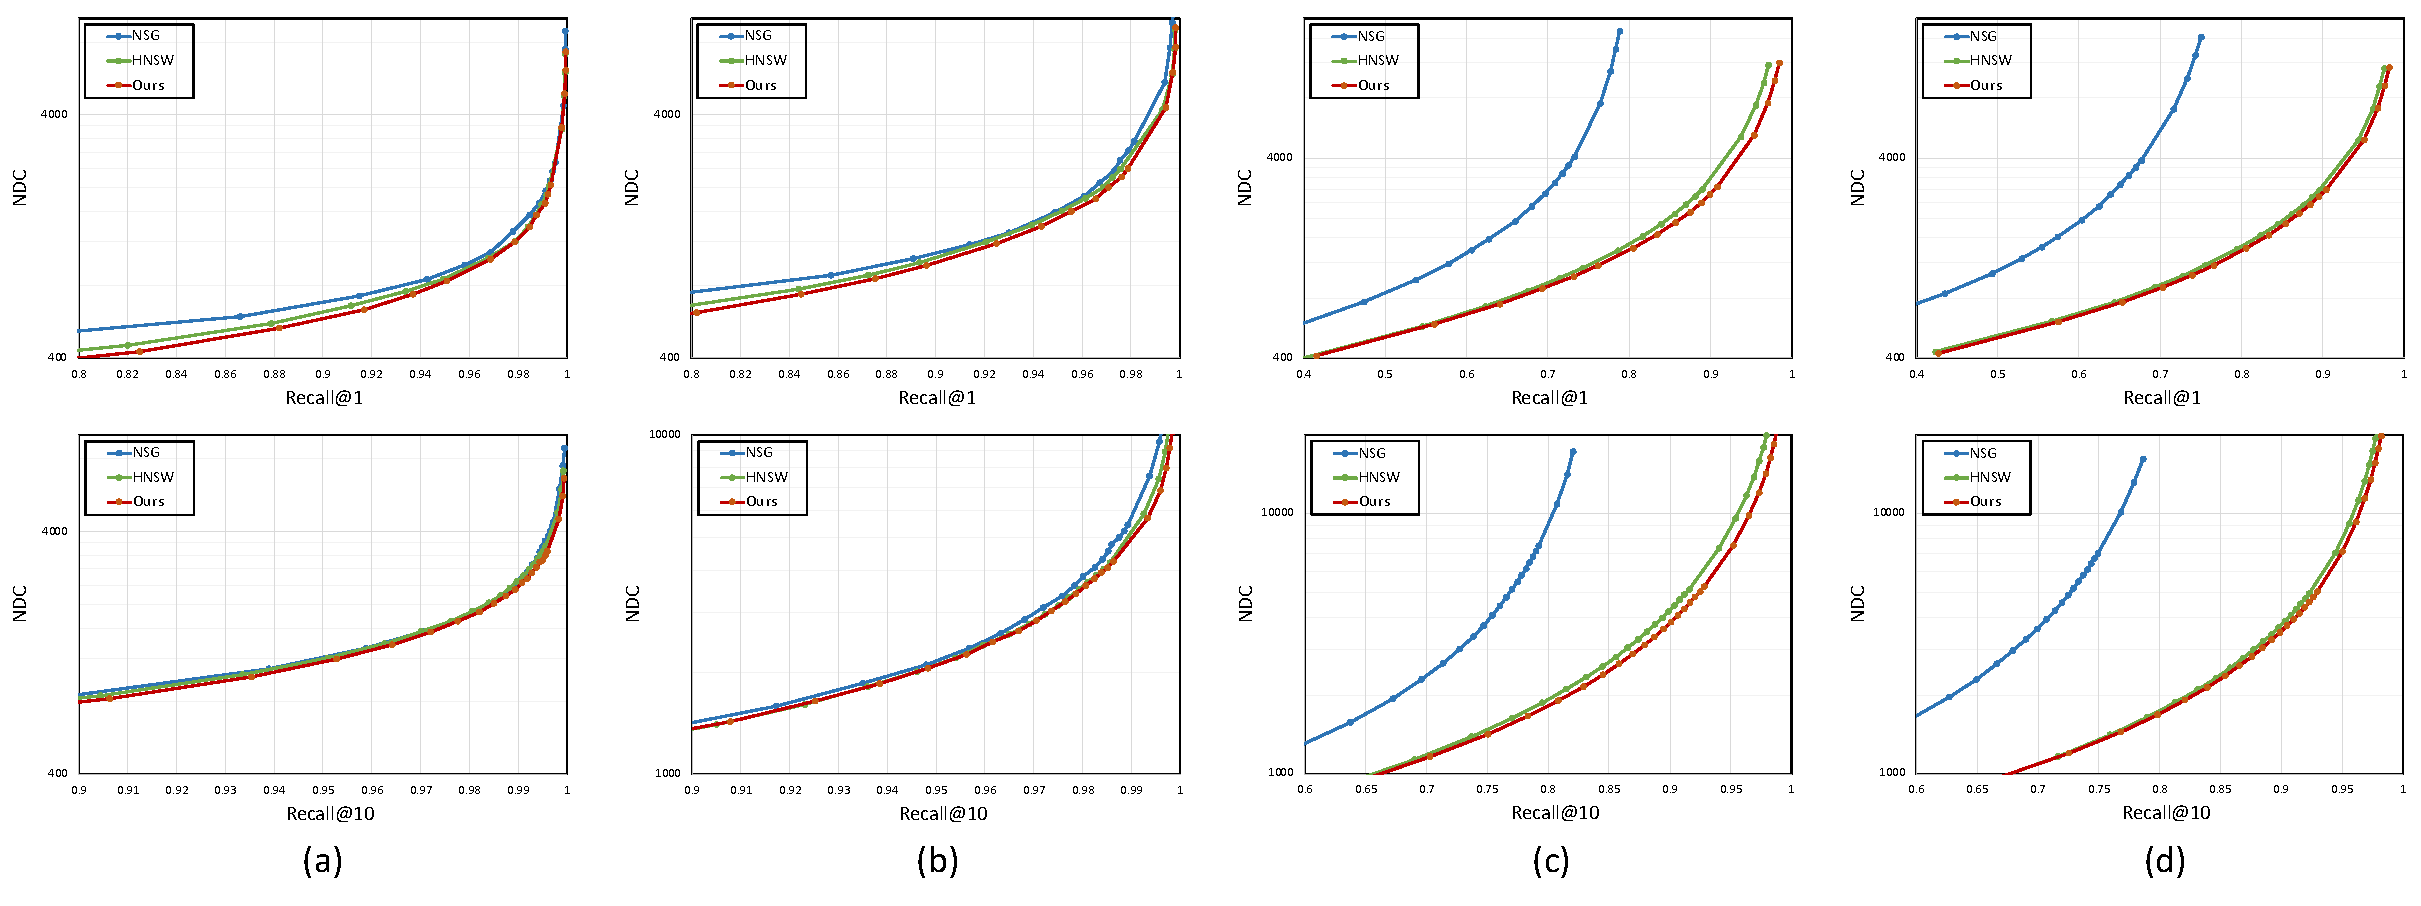
\includegraphics[width=\textwidth]{figures/context-1/exper-total.pdf}
  \caption{我们的方法分别对比HNSW和NSG算法在(a)DEEP1M,(b)DEEP10M,(c)Turing1M和(d)Turing10M 四个不同的数据集上(靠近右下更好)}
  \label{fig:exper-total}
\end{figure*}

\subsection{消融实验}
\subsubsection{反向连接增强}
在反向连接增强策略中,有两种增强模式:从候选点的随机连接部分和无法到达插入点的点。如图~\ref{fig:exper-c1}所示,我们在Turing1M数据集上将这两种策略与基线进行了比较。我们绘制了两种策略相对于基线搜索速度和基线的实际搜索速度(红色曲线)的速度。
在R@1和R@10的情况下,召回率分别为0.7、0.8和0.9。随机增强策略希望达到与基线相同的召回率,但搜索速度较慢。在R@1的情况下,我们的方法比基线分别提高了5\%,9\%和10\%的速度。这表明我们的连接增强策略在图索引上的连通性优于随机策略。
\begin{figure}[htbp]
  \centering
  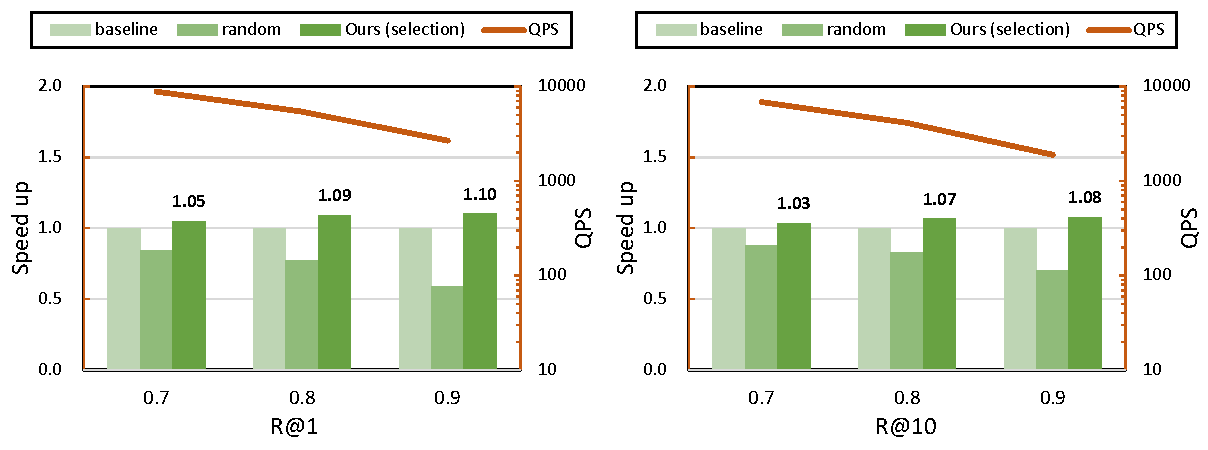
\includegraphics[width=0.7\textwidth]{figures/context-1/exper-c1.pdf}
  \caption{不同的基线反向增强和相对加速度,以及基线搜索速度。当召回率为0.9时,该策略可以加速10\%。}
  \label{fig:exper-c1}
\end{figure}


\subsubsection{查询感知策略的可扩展性}
为了证明所提出的查询感知早停策略的可扩展性,在DEEP1M和DEEP10M数据集上进行了实验。对于每个数据集,我们分别使用R@10和R@100进行实验。如表~\ref{tab:exper-c3}所示,我们分别列出了HNSW和我们的方法在DEEP数据集上实现高召回率时的NDC,以及搜索速度的比例加快。
我们发现,召回率越大,搜索速度加快的比例越大。特别地,当在DEEP1M数据集上的召回率R@10 = 0.999时,该策略可以将搜索过程加快1.29倍。在其他情况下,搜索速度有不同程度的提高。

\begin{table*}[htbp]
  \centering
  \caption{在相同召回率的情况下,采用查询感知早停策略所需的距离计算量(NDC)与基线算法的比较。}
  \label{tab:exper-c3}
  \resizebox{\textwidth}{!}{%
  \begin{tabular}{c|ccc|ccc|ccc|ccc}
  \hline
  \multirow{3}{*}{Recall rate} & \multicolumn{3}{c|}{DEEP1M-R@10} & \multicolumn{3}{c|}{DEEP1M-R@100} & \multicolumn{3}{c|}{DEEP10M-R@10} & \multicolumn{3}{c}{DEEP10M-R@100} \\ \cline{2-13} 
   & \multicolumn{2}{c}{dist.   compution} & \multirow{2}{*}{speed up} & \multicolumn{2}{c}{dist.   compution} & \multirow{2}{*}{speed up} & \multicolumn{2}{c}{dist.   compution} & \multirow{2}{*}{speed up} & \multicolumn{2}{c}{dist.   compution} & \multirow{2}{*}{speed up} \\
   & HNSW & Ours &  & HNSW & Ours &  & HNSW & Ours &  & HNSW & Ours &  \\ \hline
  0.99 & 2637.87 & 2475.86 & 1.07 & 4905.17 & 4611.04 & 1.06 & 5865.32 & 5368.36 & 1.09 & 10362.2 & 9709.18 & 1.07 \\
  0.995 & 3347.81 & 3067.41 & 1.09 & 6553.21 & 5965.97 & 1.10 & 7429.83 & 6659.18 & 1.12 & 14424.3 & 13233.8 & 1.09 \\
  0.999 & 7110.67 & 5500.62 & \textbf{1.29} & 12125.8 & 10328.2 & 1.17 & 15712.9 & 13204.6 & 1.19 & 27463.4 & 24713.9 & 1.11 \\ \hline
  \end{tabular}%
  }
\end{table*}


\section{本章小结}
本章节对\ganns 方法从近邻图角度进行了研究,指出现有方法面临的两个挑战:图连通性差和搜索存在冗余。图连通性差是由于构建算法中存在点的入度约束导致的。搜索存在冗余是由于搜索算法没有感知到查询的最小搜索步数。因此,本文提出反向连接增强策略,通过判断插入点是否可达来增加一些连接,使插入点的入度不再受限制。其次,本文提出了查询感知早停策略,通过在搜索过程中收集动态距离特征并为每个查询分配不同的搜索步数来减少搜索冗余开销。最后,通过大量实验表明,该方法可以将搜索速度提高1.06到1.29倍。
% !TeX root = ../main.tex

\chapter{面向近存架构的高效算法设计}


\section{概述}\label{sec:nmp-overview}
现有的最佳优先搜索算法在冯诺依曼架构上执行非常低效,原因是搜索算法主要的算子之一是距离计算。
计算两个向量之间的距离,由于图算法的特性,导致向量数据对于某个查询来说不存在复用,因此整个搜索算法的76.7\%的时间开销在访存上

近邻图搜索算法的算子有以下几种,分别是:距离计算、过滤、排序和索引。


\section{方法介绍}\label{sec:nmp-method}
在本节中会重点介绍本章所提出的面向近存架构的高效算法设计方法。首先介绍近邻图搜索算法的建模,指出在CPU上的距离计算操作是整个搜索算法的瓶颈。然后在\ref{sec:nmp-method-distance}节中介绍搜索算法中距离计算操作并行化的方法。当距离计算操作被并行化后,排序操作会成为限制性能进一步提升的瓶颈。最后在\ref{sec:nmp-method-sort}节介绍延迟排序策略,以实现搜索算法在近存架构上的完全流水(图~\ref{fig:software-opt}(e))。

\begin{figure}[htbp]
  \centering
  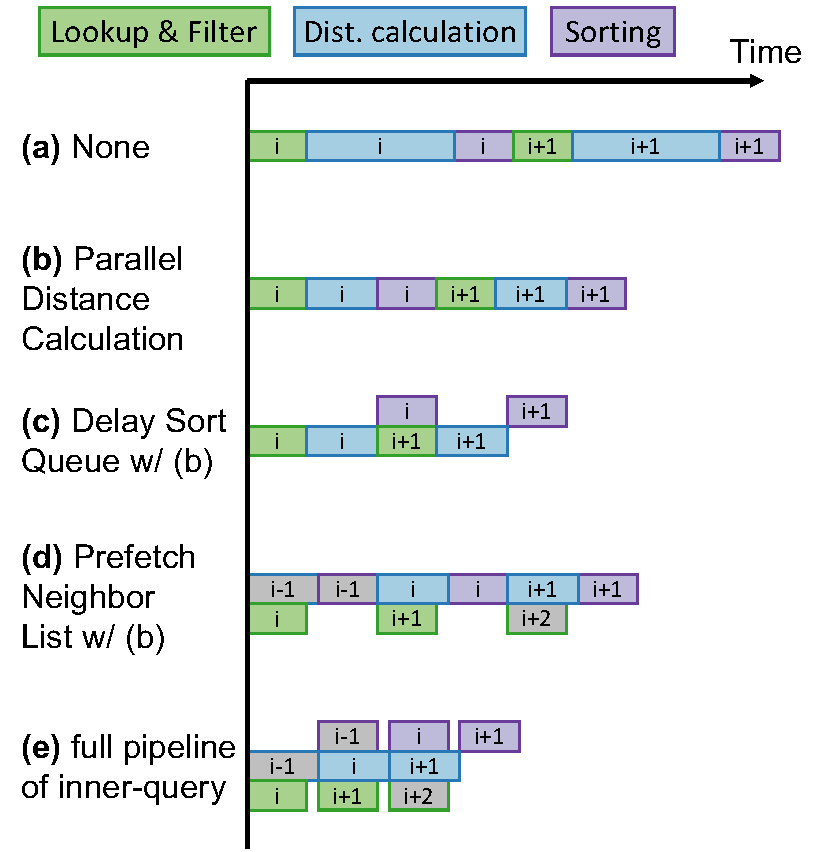
\includegraphics[width=0.45\textwidth]{figures/context-2/software-opt.pdf}
  \caption{Software solutions. \todo{Add figures}}
  \label{fig:software-opt}
\end{figure}

\subsection{近邻图搜索算法建模}\label{sec:nmp-method-model}
% 针对单机的搜索算法建模
% 合并一下我之前的模型(简化一些)+华哥列的计算表达式,突出体现有几个计算步骤,承接下面的两个技术
本节对近邻图搜索算法进行建模和分析。如前所述,对于某个查询点,它完整的搜索过程是由若干个轮次组成的,总轮次记为$\#round$。那么,整个近邻图搜索算法的执行时间可以表示为:
\begin{equation}
  T_{query}=\#iter\times \left( T_{nlist}+T_{filter}+T_{dist}+T_{sort} \right)
  \label{eq:nmp-overall}
\end{equation}

整个搜索过程包括以下四个算子:
\begin{enumerate}
  \item \textbf{取邻居列表}~根据当前搜索点,获取它的全部邻居;
  \item \textbf{过滤重复点}~由于部分邻居点已经在之前的轮次中被计算过和查询点之间的距离,为了避免重复计算,需要将这些计算过的邻居点去掉;
  \item \textbf{距离计算}~对于过滤后的邻居点,逐个计算它们和查询点之间的距离;
  \item \textbf{排序}~将本轮完成计算的邻居点,根据它们与查询点的距离,逐个添加到搜索队列中。
\end{enumerate}

相应的,

式~\ref{eq:nmp-overall}中的$T_{nlist}$表示取邻居列表的执行时间,可进一步表示为:
\begin{equation}
  T_{nlist}=\#nbor\times l_{index}\times t_{mem}
\end{equation}
其中$\#nbor$表示搜索点的邻居数量(下同),$l_{index}$表示每个邻居点所需要的存储量(例如,4字节),$t_{mem}$表示获取单位数据用于计算所需要的时间开销(下同),这一时间与实际的硬件实现方式有关。

式~\ref{eq:nmp-overall}中的$T_{filter}$表示过滤重复点的执行时间,可进一步表示为:
\begin{equation}
  T_{filter}=\#nbor\times t_{filter}
\end{equation}
其中$t_{filter}$表示过滤一个邻居点所需要的时间开销,这一时间与实际硬件和实现方式都有关,例如在CPU上可以通过查表的方式实现。

式~\ref{eq:nmp-overall}中的$T_{dist}$表示距离计算的执行时间,可进一步表示为:
\begin{equation}
  T_{dist}=\#nbor\prime \times \left(\#dim\times l_{value}\times t_{mem} + t_{calc} \right)
\end{equation}
其中$\#nbor\prime$表示搜索点过滤后的邻居数量(下同),一般与$\#nbor$相差不大,实验中平均有10\%-20\%的点会被过滤掉。$\#dim$表示数据点特征的维度,$l_{value}$表示每个维度数据所需要的存储量(例如常见的有,1字节的$int8$和$uint8$数据类型,4字节的$float32$数据类型)。$t_{mem}$的含义同上,$t_{calc}$表示计算单个点与查询距离的时间开销。由于查询点的数据是频繁被使用的,因此距离计算操作只考虑了一个向量的访存情况。

式~\ref{eq:nmp-overall}中的$T_{sort}$表示排序的执行时间,可进一步表示为:
\begin{equation}
  T_{sort}=\#nbor\prime \times t_{sort}
\end{equation}
其中$t_{sort}$表示将一个点插入到优先队列中所需要的时间开销。

基于上述的分析,本文进一步对HNSW近邻图搜索算法在CPU上的时间开销组成进行了分析。本文分别在SIFT10M和DEEP10M两个数据集上进行了测试,结果如图~\ref{fig:operation-time}所示。可以发现,距离计算是整个搜索过程中时间开销占比最大的操作,占比高达85\%以上,其次是排序操作占比在10\%左右,重复点过滤占比在5\%左右。由于取邻居列表的时间开销很小,因此归类到其他中。

\begin{figure}
  \centering
  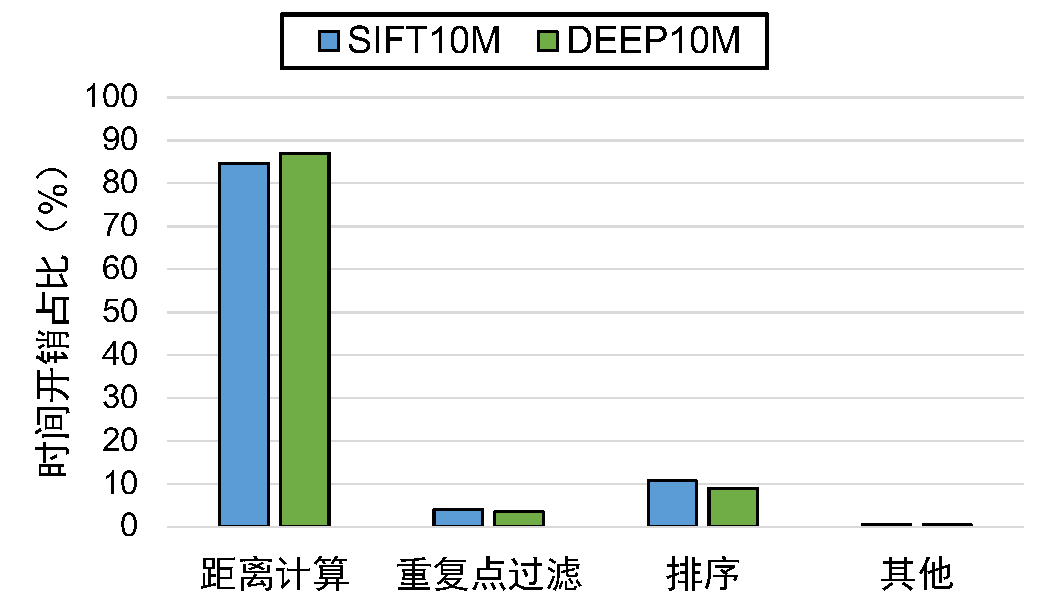
\includegraphics[width=0.6\textwidth]{figures/context-2/operation-time.pdf}
  \caption{每个操作在CPU上运行的时间开销百分比}
  \label{fig:operation-time}
\end{figure}


\subsection{面向近存的并行算法设计}\label{sec:nmp-method-distance}
% 不同的分配方法,以及过滤操作也要并行?
综上所述,近邻图搜索算法中的距离计算操作是整个计算过程的瓶颈。根据\ref{sec:nmp-method-model}节的建模不难发现,这一挑战的原因有两个:一方面,距离计算操作需要读取数据特征,因此访存量是其他操作的几十倍(例如SIFT数据集,对于某个点来说,其特征大小为128维度\times1字节,而索引大小仅为4字节;DEEP数据集单个点的特征大小为96维度\times4字节)。另一方面,搜索是根据近邻图进行的,而图这种数据结构具有天然的不规则访存的特点。上述两个问题叠加在一起,导致了近邻图搜索算法在现有冯诺依曼架构上的低效。因此,本文采用近存架构来解决这一问题。

% TODO:背景或者基础部分需要介绍一下DRAM?
为了充分发挥近存架构的潜在能力,需要设计高效的算法,将近邻图搜索映射在近存架构上。其中距离计算和重复点过滤两个操作比较容易实现并行化,因此将它们通过并行的方式在近存架构的rank层级上执行。整个图的特征是以矩阵的方式紧密存储的(即,特征矩阵),矩阵的行数就是图上的点数,矩阵的列数是数据特征的维度。因此需要将特征矩阵分成$N_r$个部分($N_r$是可供使用的rank数量,因为索引矩阵也需要一定的存储空间),以并行的方式执行距离计算操作。并行化距离计算操作的实际执行时间依赖于$N_r$中执行时间最长的那个,因此我们需要选择一个更好的映射方法(特征矩阵到子特征矩阵)。测试了两种典型的映射方法:顺序映射和模映射。顺序映射是将特征矩阵依次划分为$N_r$子特征矩阵。模映射是将特征矩阵的基向量依次划分为不同的子特征矩阵。Eq. \ref{eq:mapping}给出了这两种映射方法的计算表达式。
\begin{equation}\label{eq:mapping}
\begin{split}
L_{seq}\left(Id\right) = Id / \left \lceil N / N_r \right \rceil \\
L_{mod}\left(Id\right) = Id\ mod\ N_r
\end{split}
\end{equation}

首先分析了这两种映射方法的理论性能;如图\ref{fig:parallel-dist}(左)所示,其中$N_r=4$,由于总的计算量相同,利用率最低的子特征矩阵决定了最终距离计算的性能。与串行映射相比,模映射的性能提高了27\%。此外,我们还分析了加速比与$N_r$的关系,我们发现当$N_r=4$时,并行距离计算可以达到2.7倍的加速比(图\ref{fig:parallel-dist}(右))。因此,可以通过模映射实现距离计算的并行化。

\begin{figure}
  \centering
  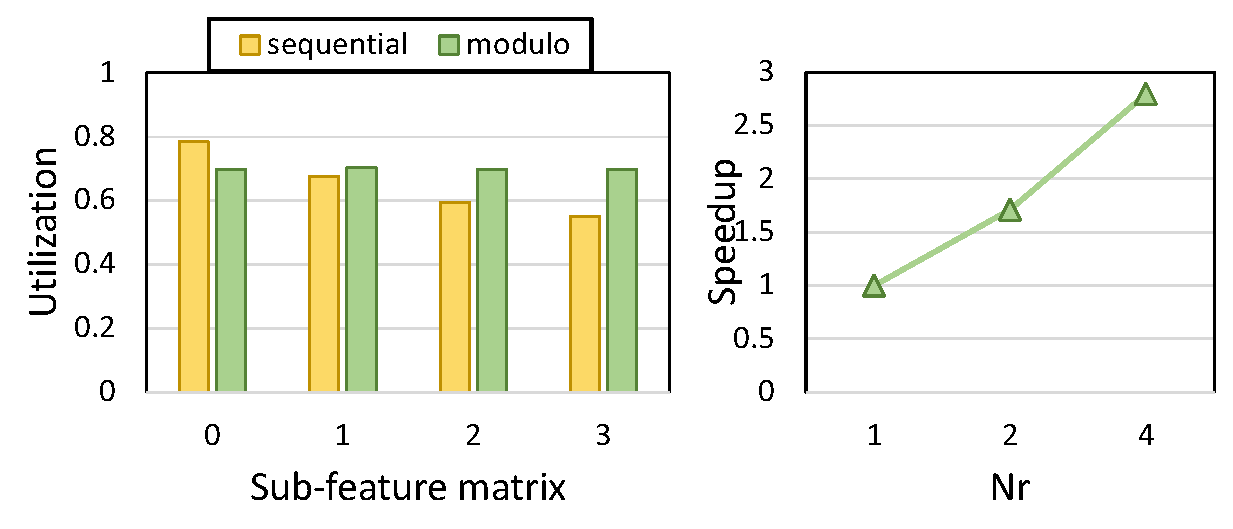
\includegraphics[width=0.9\textwidth]{figures/context-2/parallel-dist.pdf}
  \caption{左:子特征矩阵的利用率分布,最终性能取决于利用率最差的子特征矩阵。右:使用模映射方法加速比和$N_r$之间的关系。}
  \label{fig:parallel-dist}
\end{figure}

\subsection{延迟排序方法}\label{sec:nmp-method-sort}
距离计算操作并行化后,排序的时间开销不可忽视。为此,提出延迟排序队列策略来隐藏排序的时间开销。在原始的搜索算法计算流程中,$i$ -th步搜索依赖于$(i-1)$ -th排序结果,导致排序操作不能与其他操作并行执行。
经过分析,我们发现$i$-th步骤的搜索点($i>1$)只有两个来源。一个是$(i-1)$ -th步骤中最近的未搜索点,另一个是$(i-1)$ -th步骤距离计算结果中最小$Dist.$的点($Id_{dcmin}$)。根据这个特性,我们可以在距离计算操作之后无需排序操作就可以开始下一步的搜索。

我们需要添加两个更改来实现这个策略。(1)在距离计算操作中,每个子特征矩阵需要额外输出一个最小的点$Dist.$,并选择最小的点作为$Id_{dcmin}$。(2)在选择操作中,$i$ -th步骤中的搜索点只需选择$(i-2)$ -th步骤中的最近未搜索点与$(i-1)$ -th步骤中的$Id_{dcmin}$之间距离最小的搜索点。
然后,我们分析了延迟排序队列策略带来的额外开销,与并行距离计算方法相比,它仅占总运行时间的0.5\%。




\section{实验结果}\label{sec:nmp-experiment}
\subsection{实验设置}

\subsection{实现方法}
% 在FPGA上进行了验证

\subsection{整体性能}

\subsection{消融实验}




\section{本章小结}\label{sec:nmp-conclusion}



% !TeX root = ../main.tex

\chapter{面向分布式架构的高效算法设计}


\section{概述}\label{sec:dist-overview}
% 怎么拓展到Billion-Scale?现有方法怎么做的?


\section{方法介绍}\label{sec:dist-method}

\subsection{混合并行分布式算法建模}\label{sec:dist-method-model}
% 本章节的并行是针对机器的,例如是多机之间?单机内部?

\subsection{索引预先加载策略}\label{sec:dist-method-index}
% 命中率越来越高,近存那部分工作可以放在这里
最后,我们提出了预取邻居列表策略来隐藏查找和过滤操作的时间开销。为了便于描述,这里不考虑延迟排序队列策略。在原始的搜索算法计算流程中,$i$ -th步骤的距离计算操作依赖于$i$ -th步骤的邻居列表,这使得查找&过滤操作无法与其他操作并行。这里我们首先定义\textit{潜在的未搜索点}($p_{pu}$),它是队列中最小的$Dist.$和$Flag$为真的点(除了最近的未搜索点)。我们发现$(i-1)$ -th步骤的潜在未搜索点有很大的概率成为$i$ -th步骤的搜索点(我们称之为搜索命中)。为了进一步量化这一现象,我们将$n$ -th步骤中的搜索命中率定义为$(n+l)$ -th步骤。
\begin{equation}\label{eq:hit rate}
hit\ rate = \frac{1}{l}\sum\limits_{i=n+1}\limits^{n+l}{\left| p_s^{(i)} = p_{pu}^{(i-1)} \right|}
\end{equation}

如图\ref{fig:hit rate}所示,我们将搜索过程平均分成十个部分,然后分别计算每个部分的搜索命中率。实验结果表明,除前20\%的步骤外,其余80\%的步骤的平均搜索命中率为82.6\% ~ 84.1\%。也就是说,我们可以根据$(i-1)$ -th步骤的潜在未搜索点提前执行Lookup&Filter操作,以便$i$ -th步骤的距离计算操作不必等待$i$ -th步骤的Lookup&Filter操作(如果它命中)。
我们需要添加一个更改来实现这个策略。在选择操作中,我们首先确定搜索是否命中。如果没有被命中,我们需要根据搜索点重新执行查找和过滤操作。

\begin{figure}
  \centering
  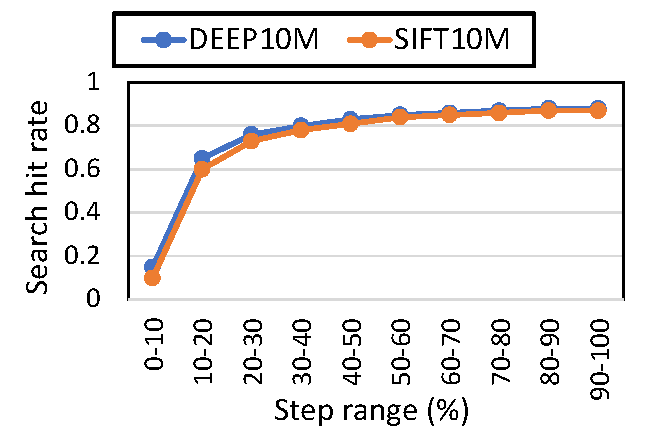
\includegraphics[width=0.5\textwidth]{figures/context-2/hitrate.pdf}
  \caption{The search hit rate varies with the search step (R@10 is 0.97). The average hit rate of the last 80\% steps is 82.6\%-84.1\%.}
  \label{fig:hitrate}
\end{figure}

\subsection{特征延迟处理策略}\label{sec:dist-method-feature}



\section{实验结果}\label{sec:dist-experiment}
\subsection{实验设置}

\subsection{实现方法}
% 在FPGA上进行了验证

\subsection{整体性能}

\subsection{消融实验}



\section{本章小结}\label{sec:dist-conclusion}

% !TeX root = ../main.tex

\chapter{论文主要部分的写法}

研究生学位论文撰写,除表达形式上需要符合一定的格式要求外,内容方面上也要遵循一些共性原则。

通常研究生学位论文只能有一个主题(不能是几块工作拼凑在一起),该主题应针对某学科领域中的一个具体问题展开深入、系统的研究,并得出有价值的研究结论。
学位论文的研究主题切忌过大,例如,“中国国有企业改制问题研究”这样的研究主题过大,因为“国企改制”涉及的问题范围太广,很难在一本研究生学位论文中完全研究透彻。



\section{论文的语言及表述}

除国际研究生外,学位论文一律须用汉语书写。
学位论文应当用规范汉字进行撰写,除古汉语研究中涉及的古文字和参考文献中引用的外文文献之外,均采用简体汉字撰写。

国际研究生一般应以中文或英文书写学位论文,格式要求同上。
论文须用中文封面。

研究生学位论文是学术作品,因此其表述要严谨简明,重点突出,专业常识应简写或不写,做到立论正确、数据可靠、说明透彻、推理严谨、文字凝练、层次分明,避免使用文学性质的或带感情色彩的非学术性语言。

论文中如出现一个非通用性的新名词、新术语或新概念,需随即解释清楚。



\section{论文题目的写法}

论文题目应简明扼要地反映论文工作的主要内容,力求精炼、准确,切忌笼统。
论文题目是对研究对象的准确、具体描述,一般要在一定程度上体现研究结论,因此,论文题目不仅应告诉读者这本论文研究了什么问题,更要告诉读者这个研究得出的结论。
例如:“在事实与虚构之间:梅乐、卡彭特、沃尔夫的新闻观”就比“三个美国作家的新闻观研究”更专业、更准确。



\section{摘要的写法}

论文摘要是对论文研究内容的高度概括,应具有独立性和自含性,即应是 一篇简短但意义完整的文章。
通过阅读论文摘要,读者应该能够对论文的研究 方法及结论有一个整体性的了解,因此摘要的写法应力求精确简明。
论文摘要 应包括对问题及研究目的的描述、对使用的方法和研究过程进行的简要介绍、 对研究结论的高度凝练等,重点是结果和结论。

论文摘要切忌写成全文的提纲,尤其要避免“第 1 章……;第 2 章……;……”这样的陈述方式。



\section{引言的写法}

一篇学位论文的引言大致包含如下几个部分:
1、问题的提出;
2、选题背 景及意义;
3、文献综述;
4、研究方法;
5、论文结构安排。
\begin{itemize}
  \item 问题的提出:要清晰地阐述所要研究的问题“是什么”。
    \footnote{选题时切记要有“问题意识”,不要选不是问题的问题来研究。}
  \item 选题背景及意义:论述清楚为什么选择这个题目来研究,即阐述该研究对学科发展的贡献、对国计民生的理论与现实意义等。
  \item 文献综述:对本研究主题范围内的文献进行详尽的综合述评,“述”的同时一定要有“评”,指出现有研究状态,仍存在哪些尚待解决的问题,讲出自己的研究有哪些探索性内容。
  \item 研究方法:讲清论文所使用的学术研究方法。
  \item 论文结构安排:介绍本论文的写作结构安排。
\end{itemize}



\section{正文的写法}

本部分是论文作者的研究内容,不能将他人研究成果不加区分地掺和进来。
已经在引言的文献综述部分讲过的内容,这里不需要再重复。
各章之间要存在有机联系,符合逻辑顺序。



\section{结论的写法}

结论是对论文主要研究结果、论点的提炼与概括,应精炼、准确、完整,使读者看后能全面了解论文的意义、目的和工作内容。
结论是最终的、总体的结论,不是正文各章小结的简单重复。
结论应包括论文的核心观点,主要阐述作者的创造性工作及所取得的研究成果在本领域中的地位、作用和意义,交代研究工作的局限,提出未来工作的意见或建议。
同时,要严格区分自己取得的成果与指导教师及他人的学术成果。

在评价自己的研究工作成果时,要实事求是,除非有足够的证据表明自己的研究是“首次”、“领先”、“填补空白”的,否则应避免使用这些或类似词语。

% !TeX root = ../main.tex

\chapter{图表示例}

\section{插图}

图片通常在 \env{figure} 环境中使用 \cs{includegraphics} 插入,如图~\ref{fig:example} 的源代码。
建议矢量图片使用 PDF 格式,比如数据可视化的绘图;
照片应使用 JPG 格式;
其他的栅格图应使用无损的 PNG 格式。
注意,LaTeX 不支持 TIFF 格式;EPS 格式已经过时。

\begin{figure}
  \centering
  \includegraphics[width=0.5\linewidth]{example-image-a.pdf}
  \caption*{国外的期刊习惯将图表的标题和说明文字写成一段,需要改写为标题只含图表的名称,其他说明文字以注释方式写在图表下方,或者写在正文中。}
  \caption{示例图片标题}
  \label{fig:example}
\end{figure}

若图或表中有附注,采用英文小写字母顺序编号,附注写在图或表的下方。
国外的期刊习惯将图表的标题和说明文字写成一段,需要改写为标题只含图表的名称,其他说明文字以注释方式写在图表下方,或者写在正文中。

如果一个图由两个或两个以上分图组成时,各分图分别以 (a)、(b)、(c)...... 作为图序,并须有分图题。
推荐使用 \pkg{subcaption} 宏包来处理, 比如图~\ref{fig:subfig-a} 和图~\ref{fig:subfig-b}。

\begin{figure}
  \centering
  \subcaptionbox{分图 A\label{fig:subfig-a}}
    {\includegraphics[width=0.35\linewidth]{example-image-a.pdf}}
  \subcaptionbox{分图 B\label{fig:subfig-b}}
    {\includegraphics[width=0.35\linewidth]{example-image-b.pdf}}
  \caption{多个分图的示例}
  \label{fig:multi-image}
\end{figure}



\section{表格}

表应具有自明性。为使表格简洁易读,尽可能采用三线表,如表~\ref{tab:three-line}。
三条线可以使用 \pkg{booktabs} 宏包提供的命令生成。

\begin{table}
  \centering
  \caption{三线表示例}
  \begin{tabular}{ll}
    \toprule
    文件名          & 描述                         \\
    \midrule
    thuthesis.dtx   & 模板的源文件,包括文档和注释 \\
    thuthesis.cls   & 模板文件                     \\
    thuthesis-*.bst & BibTeX 参考文献表样式文件    \\
    \bottomrule
  \end{tabular}
  \label{tab:three-line}
\end{table}

表格如果有附注,尤其是需要在表格中进行标注时,可以使用 \pkg{threeparttable} 宏包。
研究生要求使用英文小写字母 a、b、c……顺序编号,本科生使用圈码 ①、②、③……编号。

\begin{table}
  \centering
  \begin{threeparttable}[c]
    \caption{带附注的表格示例}
    \label{tab:three-part-table}
    \begin{tabular}{ll}
      \toprule
      文件名                 & 描述                         \\
      \midrule
      thuthesis.dtx\tnote{a} & 模板的源文件,包括文档和注释 \\
      thuthesis.cls\tnote{b} & 模板文件                     \\
      thuthesis-*.bst        & BibTeX 参考文献表样式文件    \\
      \bottomrule
    \end{tabular}
    \begin{tablenotes}
      \item [a] 可以通过 xelatex 编译生成模板的使用说明文档;
        使用 xetex 编译 \file{thuthesis.ins} 时则会从 \file{.dtx} 中去除掉文档和注释,得到精简的 \file{.cls} 文件。
      \item [b] 更新模板时,一定要记得编译生成 \file{.cls} 文件,否则编译论文时载入的依然是旧版的模板。
    \end{tablenotes}
  \end{threeparttable}
\end{table}

如某个表需要转页接排,可以使用 \pkg{longtable} 宏包,需要在随后的各页上重复表的编号。
编号后跟表题(可省略)和“(续)”,置于表上方。续表均应重复表头。

\begin{longtable}{cccc}
    \caption{跨页长表格的表题}
    \label{tab:longtable} \\
    \toprule
    表头 1 & 表头 2 & 表头 3 & 表头 4 \\
    \midrule
  \endfirsthead
    \caption*{续表~\thetable\quad 跨页长表格的表题} \\
    \toprule
    表头 1 & 表头 2 & 表头 3 & 表头 4 \\
    \midrule
  \endhead
    \bottomrule
  \endfoot
  Row 1  & & & \\
  Row 2  & & & \\
  Row 3  & & & \\
  Row 4  & & & \\
  Row 5  & & & \\
  Row 6  & & & \\
  Row 7  & & & \\
  Row 8  & & & \\
  Row 9  & & & \\
  Row 10 & & & \\
\end{longtable}



\section{算法}

算法环境可以使用 \pkg{algorithms} 或者 \pkg{algorithm2e} 宏包。

\renewcommand{\algorithmicrequire}{\textbf{输入:}\unskip}
\renewcommand{\algorithmicensure}{\textbf{输出:}\unskip}

\begin{algorithm}
  \caption{Calculate $y = x^n$}
  \label{alg1}
  \small
  \begin{algorithmic}
    \REQUIRE $n \geq 0$
    \ENSURE $y = x^n$

    \STATE $y \leftarrow 1$
    \STATE $X \leftarrow x$
    \STATE $N \leftarrow n$

    \WHILE{$N \neq 0$}
      \IF{$N$ is even}
        \STATE $X \leftarrow X \times X$
        \STATE $N \leftarrow N / 2$
      \ELSE[$N$ is odd]
        \STATE $y \leftarrow y \times X$
        \STATE $N \leftarrow N - 1$
      \ENDIF
    \ENDWHILE
  \end{algorithmic}
\end{algorithm}

% !TeX root = ../main.tex

\chapter{数学符号和公式}

\section{数学符号}

中文论文的数学符号默认遵循 GB/T 3102.11—1993《物理科学和技术中使用的数学符号》
\footnote{原 GB 3102.11—1993,自 2017 年 3 月 23 日起,该标准转为推荐性标准。}。
该标准参照采纳 ISO 31-11:1992 \footnote{目前已更新为 ISO 80000-2:2019。},
但是与 \TeX{} 默认的美国数学学会(AMS)的符号习惯有所区别。
具体地来说主要有以下差异:
\begin{enumerate}
  \item 大写希腊字母默认为斜体,如
    \begin{equation*}
      \Gamma \Delta \Theta \Lambda \Xi \Pi \Sigma \Upsilon \Phi \Psi \Omega.
    \end{equation*}
    注意有限增量符号 $\increment$ 固定使用正体,模板提供了 \cs{increment} 命令。
  \item 小于等于号和大于等于号使用倾斜的字形 $\le$、$\ge$。
  \item 积分号使用正体,比如 $\int$、$\oint$。
  \item
    偏微分符号 $\partial$ 使用正体。
  \item
    省略号 \cs{dots} 按照中文的习惯固定居中,比如
    \begin{equation*}
      1, 2, \dots, n \quad 1 + 2 + \dots + n.
    \end{equation*}
  \item
    实部 $\Re$ 和虚部 $\Im$ 的字体使用罗马体。
\end{enumerate}

以上数学符号样式的差异可以在模板中统一设置。
另外国标还有一些与 AMS 不同的符号使用习惯,需要用户在写作时进行处理:
\begin{enumerate}
  \item 数学常数和特殊函数名用正体,如
    \begin{equation*}
      \uppi = 3.14\dots; \quad
      \symup{i}^2 = -1; \quad
      \symup{e} = \lim_{n \to \infty} \left( 1 + \frac{1}{n} \right)^n.
    \end{equation*}
  \item 微分号使用正体,比如 $\dif y / \dif x$。
  \item 向量、矩阵和张量用粗斜体(\cs{symbf}),如 $\symbf{x}$、$\symbf{\Sigma}$、$\symbfsf{T}$。
  \item 自然对数用 $\ln x$ 不用 $\log x$。
\end{enumerate}


英文论文的数学符号使用 \TeX{} 默认的样式。
如果有必要,也可以通过设置 \verb|math-style| 选择数学符号样式。

关于量和单位推荐使用
\href{http://mirrors.ctan.org/macros/latex/contrib/siunitx/siunitx.pdf}{\pkg{siunitx}}
宏包,
可以方便地处理希腊字母以及数字与单位之间的空白,
比如:
\SI{6.4e6}{m},
\SI{9}{\micro\meter},
\si{kg.m.s^{-1}},
\SIrange{10}{20}{\degreeCelsius}。



\section{数学公式}

数学公式可以使用 \env{equation} 和 \env{equation*} 环境。
注意数学公式的引用应前后带括号,通常使用 \cs{eqref} 命令,比如式\eqref{eq:example}。
\begin{equation}
  \frac{1}{2 \uppi \symup{i}} \int_\gamma f = \sum_{k=1}^m n(\gamma; a_k) \mathscr{R}(f; a_k).
  \label{eq:example}
\end{equation}

多行公式尽可能在“=”处对齐,推荐使用 \env{align} 环境。
\begin{align}
  a & = b + c + d + e \\
    & = f + g
\end{align}



\section{数学定理}

定理环境的格式可以使用 \pkg{amsthm} 或者 \pkg{ntheorem} 宏包配置。
用户在导言区载入这两者之一后,模板会自动配置 \env{thoerem}、\env{proof} 等环境。

\begin{theorem}[Lindeberg--Lévy 中心极限定理]
  设随机变量 $X_1, X_2, \dots, X_n$ 独立同分布, 且具有期望 $\mu$ 和有限的方差 $\sigma^2 \ne 0$,
  记 $\bar{X}_n = \frac{1}{n} \sum_{i+1}^n X_i$,则
  \begin{equation}
    \lim_{n \to \infty} P \left(\frac{\sqrt{n} \left( \bar{X}_n - \mu \right)}{\sigma} \le z \right) = \Phi(z),
  \end{equation}
  其中 $\Phi(z)$ 是标准正态分布的分布函数。
\end{theorem}
\begin{proof}
  Trivial.
\end{proof}

同时模板还提供了 \env{assumption}、\env{definition}、\env{proposition}、
\env{lemma}、\env{theorem}、\env{axiom}、\env{corollary}、\env{exercise}、
\env{example}、\env{remar}、\env{problem}、\env{conjecture} 这些相关的环境。

% !TeX root = ../main.tex

\chapter{引用文献的标注}

模板支持 BibTeX 和 BibLaTeX 两种方式处理参考文献。
下文主要介绍 BibTeX 配合 \pkg{natbib} 宏包的主要使用方法。


\section{顺序编码制}

在顺序编码制下,默认的 \cs{cite} 命令同 \cs{citep} 一样,序号置于方括号中,
引文页码会放在括号外。
统一处引用的连续序号会自动用短横线连接。

\thusetup{
  cite-style = super,
}
\begin{tabular}{l@{\quad$\Rightarrow$\quad}l}
  \verb|\cite{zhangkun1994}|               & \cite{zhangkun1994}               \\
  \verb|\citet{zhangkun1994}|              & \citet{zhangkun1994}              \\
  \verb|\citep{zhangkun1994}|              & \citep{zhangkun1994}              \\
  \verb|\cite[42]{zhangkun1994}|           & \cite[42]{zhangkun1994}           \\
  \verb|\cite{zhangkun1994,zhukezhen1973}| & \cite{zhangkun1994,zhukezhen1973} \\
\end{tabular}


也可以取消上标格式,将数字序号作为文字的一部分。
建议全文统一使用相同的格式。

\thusetup{
  cite-style = inline,
}
\begin{tabular}{l@{\quad$\Rightarrow$\quad}l}
  \verb|\cite{zhangkun1994}|               & \cite{zhangkun1994}               \\
  \verb|\citet{zhangkun1994}|              & \citet{zhangkun1994}              \\
  \verb|\citep{zhangkun1994}|              & \citep{zhangkun1994}              \\
  \verb|\cite[42]{zhangkun1994}|           & \cite[42]{zhangkun1994}           \\
  \verb|\cite{zhangkun1994,zhukezhen1973}| & \cite{zhangkun1994,zhukezhen1973} \\
\end{tabular}



\section{著者-出版年制}

著者-出版年制下的 \cs{cite} 跟 \cs{citet} 一样。

\thusetup{
  cite-style = author-year,
}
\begin{tabular}{l@{\space$\Rightarrow$\space}l}
  \verb|\cite{zhangkun1994}|                & \cite{zhangkun1994}                \\
  \verb|\citet{zhangkun1994}|               & \citet{zhangkun1994}               \\
  \verb|\citep{zhangkun1994}|               & \citep{zhangkun1994}               \\
  \verb|\cite[42]{zhangkun1994}|            & \cite[42]{zhangkun1994}            \\
  \verb|\citep{zhangkun1994,zhukezhen1973}| & \citep{zhangkun1994,zhukezhen1973} \\
\end{tabular}

\vskip 2ex
\thusetup{
  cite-style = super,
}
注意,引文参考文献的每条都要在正文中标注
\cite{zhangkun1994,zhukezhen1973,dupont1974bone,zhengkaiqing1987,%
  jiangxizhou1980,jianduju1994,merkt1995rotational,mellinger1996laser,%
  bixon1996dynamics,mahui1995,carlson1981two,taylor1983scanning,%
  taylor1981study,shimizu1983laser,atkinson1982experimental,%
  kusch1975perturbations,guangxi1993,huosini1989guwu,wangfuzhi1865songlun,%
  zhaoyaodong1998xinshidai,biaozhunhua2002tushu,chubanzhuanye2004,%
  who1970factors,peebles2001probability,baishunong1998zhiwu,%
  weinstein1974pathogenic,hanjiren1985lun,dizhi1936dizhi,%
  tushuguan1957tushuguanxue,aaas1883science,fugang2000fengsha,%
  xiaoyu2001chubanye,oclc2000about,scitor2000project%
}。



% 其他部分
\backmatter

% 参考文献
\bibliography{ref/refs}  % 参考文献使用 BibTeX 编译
% \printbibliography       % 参考文献使用 BibLaTeX 编译

% 附录
% 本科生需要将附录放到声明之后,个人简历之前
\appendix
% % !TeX root = ../main.tex

\begin{survey}
\label{cha:survey}

\title{Title of the Survey}
\maketitle


\tableofcontents


本科生的外文资料调研阅读报告。


\section{Figures and Tables}

\subsection{Figures}

An example figure in appendix (Figure~\ref{fig:appendix-survey-figure}).

\begin{figure}
  \centering
  \includegraphics[width=0.6\linewidth]{example-image-a.pdf}
  \caption{Example figure in appendix}
  \label{fig:appendix-survey-figure}
\end{figure}


\subsection{Tables}

An example table in appendix (Table~\ref{tab:appendix-survey-table}).

\begin{table}
  \centering
  \caption{Example table in appendix}
  \begin{tabular}{ll}
    \toprule
    File name       & Description                                         \\
    \midrule
    thuthesis.dtx   & The source file including documentaion and comments \\
    thuthesis.cls   & The template file                                   \\
    thuthesis-*.bst & BibTeX styles                                       \\
    thuthesis-*.bbx & BibLaTeX styles for bibliographies                  \\
    thuthesis-*.cbx & BibLaTeX styles for citations                       \\
    \bottomrule
  \end{tabular}
  \label{tab:appendix-survey-table}
\end{table}


\section{Equations}

An example equation in appendix (Equation~\eqref{eq:appendix-survey-equation}).
\begin{equation}
  \frac{1}{2 \uppi \symup{i}} \int_\gamma f = \sum_{k=1}^m n(\gamma; a_k) \mathscr{R}(f; a_k)
  \label{eq:appendix-survey-equation}
\end{equation}


\section{Citations}

Example citations in appendix.
\cite{abrahams99tex}
\cite{salomon1995advanced}
\cite{abrahams99tex,salomon1995advanced}


\bibliographystyle{unsrtnat}
\bibliography{ref/appendix}

\end{survey}
       % 本科生:外文资料的调研阅读报告
% % !TeX root = ../main.tex

\begin{translation}
\label{cha:translation}

\title{书面翻译题目}
\maketitle

\tableofcontents


本科生的外文资料书面翻译。


\section{图表示例}

\subsection{图}

附录中的图片示例(图~\ref{fig:appendix-translation-figure})。

\begin{figure}
  \centering
  \includegraphics[width=0.6\linewidth]{example-image-a.pdf}
  \caption{附录中的图片示例}
  \label{fig:appendix-translation-figure}
\end{figure}


\subsection{表格}

附录中的表格示例(表~\ref{tab:appendix-translation-table})。

\begin{table}
  \centering
  \caption{附录中的表格示例}
  \begin{tabular}{ll}
    \toprule
    文件名          & 描述                         \\
    \midrule
    thuthesis.dtx   & 模板的源文件,包括文档和注释 \\
    thuthesis.cls   & 模板文件                     \\
    thuthesis-*.bst & BibTeX 参考文献表样式文件    \\
    thuthesis-*.bbx & BibLaTeX 参考文献表样式文件  \\
    thuthesis-*.cbx & BibLaTeX 引用样式文件        \\
    \bottomrule
  \end{tabular}
  \label{tab:appendix-translation-table}
\end{table}


\section{数学公式}

附录中的数学公式示例(公式\eqref{eq:appendix-translation-equation})。
\begin{equation}
  \frac{1}{2 \uppi \symup{i}} \int_\gamma f = \sum_{k=1}^m n(\gamma; a_k) \mathscr{R}(f; a_k)
  \label{eq:appendix-translation-equation}
\end{equation}


\section{文献引用}

文献引用示例\cite{abrahams99tex}。


\appendix

\section{附录}

附录的内容。


% 书面翻译的参考文献
\bibliographystyle{unsrtnat}
\bibliography{ref/appendix}

% 书面翻译对应的原文索引
\begin{translation-index}
  \nocite{salomon1995advanced}
  \bibliographystyle{unsrtnat}
  \bibliography{ref/appendix}
\end{translation-index}

\end{translation}
  % 本科生:外文资料的书面翻译
% !TeX root = ../main.tex

\chapter{补充内容}

附录是与论文内容密切相关、但编入正文又影响整篇论文编排的条理和逻辑性的资料,例如某些重要的数据表格、计算程序、统计表等,是论文主体的补充内容,可根据需要设置。


\section{图表示例}

\subsection{图}

附录中的图片示例(图~\ref{fig:appendix-figure})。

\begin{figure}
  \centering
  \includegraphics[width=0.6\linewidth]{example-image-a.pdf}
  \caption{附录中的图片示例}
  \label{fig:appendix-figure}
\end{figure}


\subsection{表格}

附录中的表格示例(表~\ref{tab:appendix-table})。

\begin{table}
  \centering
  \caption{附录中的表格示例}
  \begin{tabular}{ll}
    \toprule
    文件名          & 描述                         \\
    \midrule
    thuthesis.dtx   & 模板的源文件,包括文档和注释 \\
    thuthesis.cls   & 模板文件                     \\
    thuthesis-*.bst & BibTeX 参考文献表样式文件    \\
    thuthesis-*.bbx & BibLaTeX 参考文献表样式文件  \\
    thuthesis-*.cbx & BibLaTeX 引用样式文件        \\
    \bottomrule
  \end{tabular}
  \label{tab:appendix-table}
\end{table}


\section{数学公式}

附录中的数学公式示例(公式\eqref{eq:appendix-equation})。
\begin{equation}
  \frac{1}{2 \uppi \symup{i}} \int_\gamma f = \sum_{k=1}^m n(\gamma; a_k) \mathscr{R}(f; a_k)
  \label{eq:appendix-equation}
\end{equation}


% 致谢
% !TeX root = ../main.tex

\begin{acknowledgements}
  衷心感谢导师×××教授和物理系××副教授对本人的精心指导。他们的言传身教将使我终生受益。

  在美国麻省理工学院化学系进行九个月的合作研究期间,承蒙 Robert Field 教授热心指导与帮助,不胜感激。

  感谢×××××实验室主任×××教授,以及实验室全体老师和同窗们学的热情帮助和支持!

  本课题承蒙国家自然科学基金资助,特此致谢。
\end{acknowledgements}


% 声明
\statement
% 将签字扫描后的声明文件 scan-statement.pdf 替换原始页面
% \statement[file=scan-statement.pdf]
% 本科生编译生成的声明页默认不加页脚,插入扫描版时再补上;
% 研究生编译生成时有页眉页脚,插入扫描版时不再重复。
% 也可以手动控制是否加页眉页脚
% \statement[page-style=empty]
% \statement[file=scan-statement.pdf, page-style=plain]

% 个人简历、在学期间完成的相关学术成果
% 本科生可以附个人简历,也可以不附个人简历
% !TeX root = ../main.tex

\begin{resume}

  \section*{个人简历}

  197× 年 ×× 月 ×× 日出生于四川××县。

  1992 年 9 月考入××大学化学系××化学专业,1996 年 7 月本科毕业并获得理学学士学位。

  1996 年 9 月免试进入清华大学化学系攻读××化学博士至今。


  \section*{在学期间完成的相关学术成果}

  \subsection*{学术论文}

  \begin{achievements}
    \item Yang Y, Ren T L, Zhang L T, et al. Miniature microphone with silicon-based ferroelectric thin films[J]. Integrated Ferroelectrics, 2003, 52:229-235.
    \item 杨轶, 张宁欣, 任天令, 等. 硅基铁电微声学器件中薄膜残余应力的研究[J]. 中国机械工程, 2005, 16(14):1289-1291.
    \item 杨轶, 张宁欣, 任天令, 等. 集成铁电器件中的关键工艺研究[J]. 仪器仪表学报, 2003, 24(S4):192-193.
    \item Yang Y, Ren T L, Zhu Y P, et al. PMUTs for handwriting recognition. In press[J]. (已被Integrated Ferroelectrics录用)
  \end{achievements}


  \subsection*{专利}

  \begin{achievements}
    \item 任天令, 杨轶, 朱一平, 等. 硅基铁电微声学传感器畴极化区域控制和电极连接的方法: 中国, CN1602118A[P]. 2005-03-30.
    \item Ren T L, Yang Y, Zhu Y P, et al. Piezoelectric micro acoustic sensor based on ferroelectric materials: USA, No.11/215, 102[P]. (美国发明专利申请号.)
  \end{achievements}

\end{resume}


% 指导教师/指导小组评语
% 本科生不需要
% !TeX root = ../main.tex

\begin{comments}
% \begin{comments}[name = {指导小组评语}]
% \begin{comments}[name = {Comments from Thesis Supervisor}]
% \begin{comments}[name = {Comments from Thesis Supervision Committee}]

  论文提出了……

\end{comments}


% 答辩委员会决议书
% 本科生不需要
% !TeX root = ../main.tex

\begin{resolution}

  论文提出了……

  论文取得的主要创新性成果包括:

  1. ……

  2. ……

  3. ……

  论文工作表明作者在×××××具有×××××知识,具有××××能力,论文××××,答辩××××。

  答辩委员会表决,(×票/一致)同意通过论文答辩,并建议授予×××(姓名)×××(门类)学博士/硕士学位。

\end{resolution}


% 本科生的综合论文训练记录表(扫描版)
% \record{file=scan-record.pdf}

\end{document}
